\documentclass[preprint,5p,times,twocolumn]{elsarticle}

%\usepackage[toc,page]{appendix}
\usepackage{hyperref}
\usepackage[ruled,vlined]{algorithm2e}
%\usepackage{algorithm2e}
\usepackage{graphicx}
\usepackage{wrapfig}
\usepackage{color}
\usepackage{multirow}
%\usepackage{amsfonts}
%\usepackage{enumerate}
%\usepackage{algorithm}
\usepackage{algorithmic}
\newcommand{\jw}[1]{{\color{cyan}[[JW: #1]]}}
\newcommand{\jj}[1]{{\color{blue}[[JJ: #1]]}}
\newcommand{\jz}[1]{{\color{green}[[Jz: #1]]}}
\newcommand{\jianliu}[1]{{\color{yellow}[[JL: #1]]}}
\newcommand{\re}[1]{{\color{red} #1 }}
\newcommand{\bl}[1]{{\color{blue} #1 }}

\newcommand{\etc}{\emph{etc.}}
\newcommand{\eg}{\emph{e.g.}}
\newcommand{\etal}{\emph{et al.}}
\newcommand{\ie}{\emph{i.e. }}
\newcommand{\vs}{\emph{vs.}}
\newcommand{\eq}{\emph{Equation}}
\newcommand{\fig}{Fig.}
\newcommand{\tab}{Tab.}

\graphicspath{{figures/}}

\journal{Computer \& Graphics}

\begin{document}

\begin{frontmatter}

\title{Point Cloud Normal Estimation via Low-Rank Subspace Clustering}
\author[label1]{Jie Zhang}
\author[label1]{Junjie Cao}
\author[label1]{Xiuping Liu}
\author[label2]{Jun Wang}
\author[label1]{Jian Liu}
\author[label3]{Xiquan Shi}
\address[label1]{School of Mathematical Sciences, Dalian University of Technology, China}
\address[label2]{College of Mechanical and Electrical Engineering, Nanjing University of Aeronautics and Astronautics, China}
\address[label3]{Department of Mathematical Sciences, Delaware State University, USA}

\begin{abstract}
In this paper, we present a robust normal estimation algorithm based on the low-rank subspace clustering technique. The main idea is based on the observation that compared with the points \emph{around sharp features}, it is relatively easier to obtain accurate normals for the points \emph{within smooth regions}. The points around sharp features and smooth regions are identified by covariance analysis of their neighborhoods. The neighborhood of a point in a smooth region can be well approximated by a plane. For a point around sharp features, some of its neighbors may be in smooth regions. These neighbor points' normals are estimated by principal component analysis, and used as prior knowledge to carry out neighborhood clustering. An unsupervised learning process is designed to represent the prior knowledge as a guiding matrix. Then we segment the anisotropic neighborhood into several isotropic neighborhoods by low-rank subspace clustering with the guiding matrix, and identify a consistent subneighborhood for the current point. Hence the normal of the current point near sharp features is estimated as the normal of a plane fitting the consistent subneighborhood. Our method is capable of estimating normals accurately even in the presence of noise and anisotropic samplings, while preserving sharp features within the original point data. We demonstrate the effectiveness and robustness of the proposed method on a variety of examples.

\end{abstract}

\begin{keyword}
normal estimation \sep sharp feature preserving \sep low-rank representation \sep subspace clustering
\end{keyword}

\end{frontmatter}


%-------------------------------------------------------------------------
\section{Introduction}
Estimating surface normals from a noisy
point cloud benefits many applications in computer graphics, geometry
processing and reverse engineering. Accurate normal estimation allows a better reconstructing and rendering of point-based
surfaces \cite{DBLP:journals/cgf/OtireliGG09,DBLP:conf/siggraph/RusinkiewiczL00,WangGYTZ12,wangjun_cgf13}, anisotropic smoothing \cite{DBLP:journals/cagd/LangeP05} to name just a few.

With the assumption that the underlying surface is smooth everywhere, regression-based techniques \cite{DBLP:conf/siggraph/HoppeDDMS92,GuennebaudG07,CazalsP05,MitraNG04} use the whole neighborhoods to estimate normals. However, when a point is near sharp features, its neighborhood may be anisotropic and sampled from several piecewise surfaces.
In such case, all regression-based methods tend to smooth sharp features, since the normal estimation of the point may be influenced by its neighbors lying on some other surfaces.
%
To estimate normals more faithfully for point clouds with sharp features, Li \etal \cite{DBLP:journals/cg/LiSKCDJ10} (RNE) employed the robust statistics to classify points around sharp features into consistent sub-neighbors represented by different tangent planes.
%
However, this method is sensitive to the density variation, as shown in the bottom row of \fig \ref{fig:example}. Boulch \etal \cite{DBLP:journals/cgf/BoulchM12} (HF) introduced a uniform sampling strategy to overcome the influence of density variation.
%
However, the computed normals are unreliable for the points near sharp features, as shown in \fig \ref{fig:example}.
%
Moreover, this method tends to blur a sharp feature when the dihedral angel is large.
%
\begin{figure*}[htbp]
\begin{center}
    \begin{tabular}{c c c}
        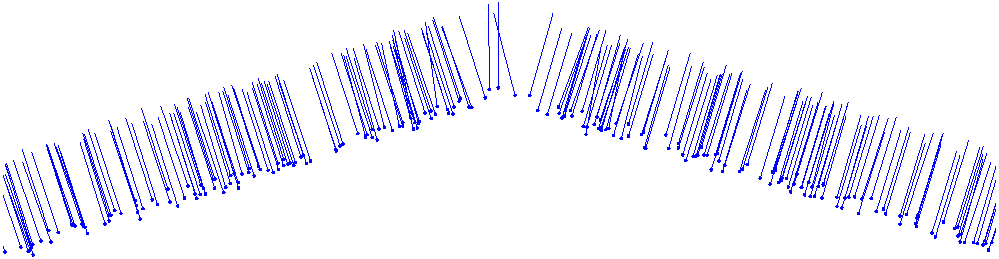
\includegraphics[width=0.3\linewidth]{example7_rne} &
        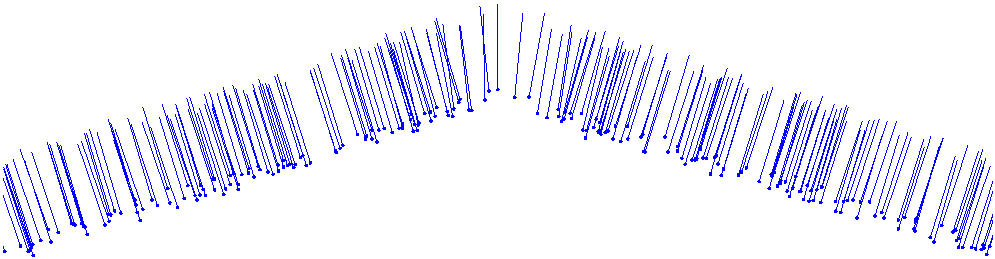
\includegraphics[width=0.3\linewidth]{example7_hf} &
        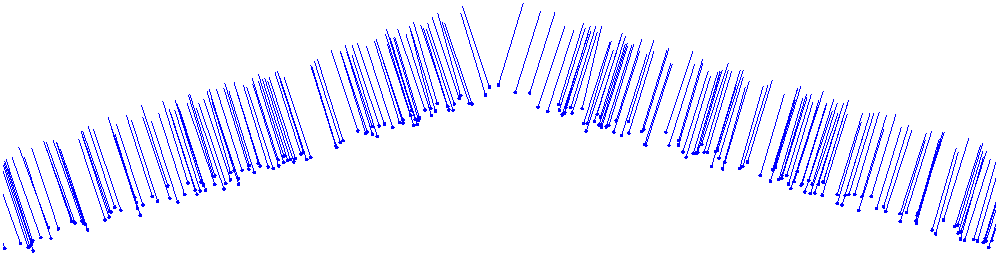
\includegraphics[width=0.3\linewidth]{example7_our}\\
        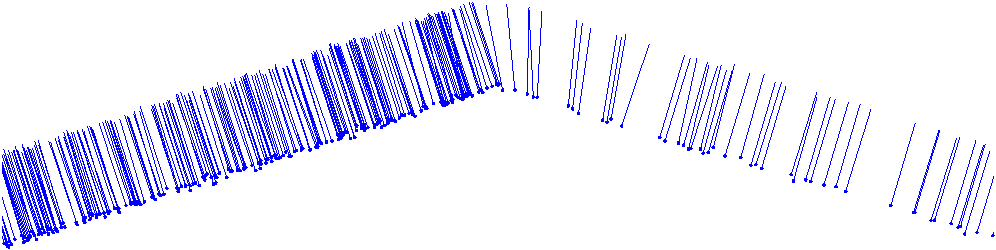
\includegraphics[width=0.3\linewidth]{example6_rne} &
        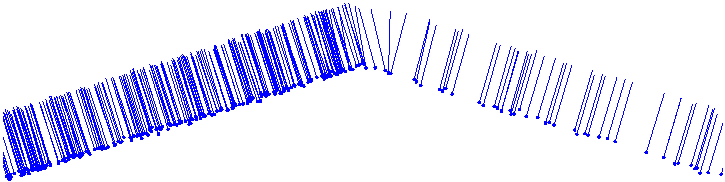
\includegraphics[width=0.3\linewidth]{example6_hf} &
        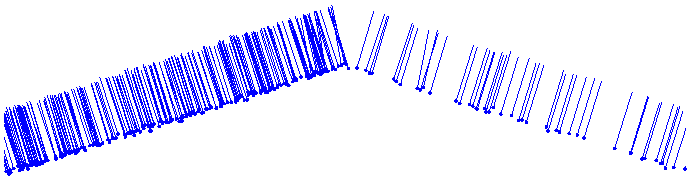
\includegraphics[width=0.3\linewidth]{example6_our}
    \end{tabular}
    \caption{\label{fig:example}
    Reconstructed normals of two plans with shallow angle by Li~\etal~\cite{DBLP:journals/cg/LiSKCDJ10} (left), Boulch~\etal~\cite{DBLP:journals/cgf/BoulchM12} (middle) and our algorithm (right). respectively.
    The points are sampled uniformly in the top row and non-uniformly in the bottom row.
    }
\end{center}
\end{figure*}

When a point is extremely near a sharp feature, it is hard to estimate its normal or classify its neighbors faithfully only by using the distance information.
%
To overcome this challenge, we present a novel robust approach to select a consistent neighborhood utilizing the structure of the underlying piecewise surfaces.
%
These surfaces can be approximated by planes and each of them is a 2D subspace, relative to the 3D Euclidean space where the model is embedded.
Thus, the segmentation of the neighborhood of a point can be solved as a subspace clustering problem, which has widespread applications in computer vision.
%
The Low-Rank Representation (LRR), emerging in machine learning, is a powerful tool in subspace clustering \cite{DBLP:journals/corr/abs-1010-2955,LiuLY10}.
It captures the global structure of the data robustly assuming that the subspaces are independent.
%
For our problem, the subspaces near sharp features are dependent, \ie the sum of the dimension of these subspaces is larger than three.
The standard low-rank method tends to fail for such case.
%
Hence we present a new low-rank subspace clustering framework with prior knowledge to handle more general subspace clustering.
In addition, we observe that the computation of normals which are not near sharp features (i.e. smooth regions) are reliable even with traditional regression-based methods, such as PCA.
%
Based on this observation, we design an unsupervised learning process to estimate the guidance from reliable regions. \re{Although it is relatively time-consuming, the consistent neighbors of a point can be effectively detected even in the presence of noise, which has many applications, including normal estimation and feature extraction,~\etc.} \fig~\ref{fig:flow_chart} gives the pipeline of our method.
The contributions of our work are summarized as follows:
\begin{itemize}
  \item The standard LRR model can only work under the assumption that the data are sampled from multiple independent subspaces. We provide a new low-rank subspace clustering framework with prior knowledge (LRSCPK) for more general subspace clustering. The prior knowledge can be obtained by many ways for different applications.
  %The standard LRR model can only work under the assumption that the data are sampled from multiple independent subspaces. By enforcing explicit structural constraint for the representation matrix, we provide a new method, named Structure Constrained LRR (SCLRR) for more general disjoint subspace clustering.
  \item For normal estimation, we use LRSCPK to segment and identify consistent subneighborhood and compute accurate normal from the subneighborhood.
      An unsupervised learning process is designed to estimate the prior knowledge from reliable regions, which are utilized in LRSCPK to classify unreliable regions close, even extremely close to sharp features.
       The estimated normals preserve sharp features even in the presence of noise and anisotropic samplings.

%  \item The sub-neighborhoods generated are useful in many applications, and we demonstrate how to use it for robust normal estimation and feature detection. I do not think the sub-neighborhood itself is useful. So the contributions should be completely re-written. I think there are two contributions: 1) the new subspace clustering method; 2) the feature-preserving normal estimation method.
\end{itemize}
%

\section{Related work}
\begin{figure*}[htbp]
  \centering
  % Requires \usepackage{graphicx}
  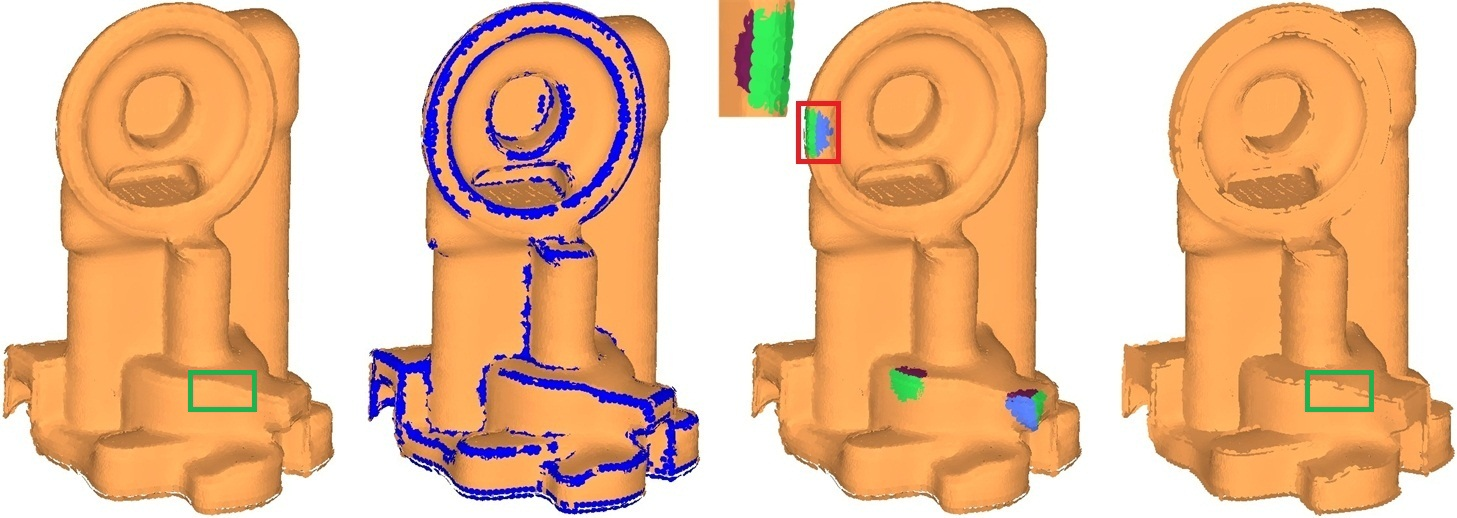
\includegraphics[width=1\linewidth]{oilpump_zj}\\
  \hspace{0 mm} (a) \hspace{38 mm} (b) \hspace{38 mm} (c)\hspace{38 mm} (d)
  \caption{Method overview.
         (a) The oil pump module with the normal computed by PCA. (b) Initial detected candidate feature points. (c) The classified subneighborhoods. The neighborhood within the red box contains three subneighborhoods rendered in blue, green and brown and the zoomed view is from left. (d) Estimated normals. Comparing (a) with (d), our method preserves the sharp features better, and the $RMS\_\tau$ introduced in section 5 is 0.6716 and 0.1308, respectively.} \label{fig:flow_chart}
\end{figure*}
%\subsection{Normal estimation}
Given a 3D point cloud, how to accurately estimate normals has been a primary concern in visual computing community. We briefly review it in this section.
%
We do not address the problem of normal orientation, which can be done separately \cite{CaoHLLS11, wang_vc12, seversky_smi11, LiuWang-SMI10, Huang-TOG09}.

%%%%%%%%%%%%%%%%%%%%%%%%%%%%%%%%%%%%%%%%%%%%%%%%%%%%%%%%%%%%%%%%%%%%%%%%%%%%%%%%%%%%%%%%%%%%%%%%%%%%%%%%%%%%
%%%%%%%%%%%%%%%%%%%%%%%%%%%%%%%%%%%%%%%%%%%%%%%%%%%%%%%%%%%%%%%%%%%%%%%%%%%%%%%%%%%%%%%%%%%%%%%%%%%%%%%%%%%%

The classical normal estimation method, proposed by Hoppe \etal \cite{DBLP:conf/siggraph/HoppeDDMS92} (PCA), defines the normal of a point as the eigenvector corresponding to the smallest eigenvalue of the covariance matrix of its neighbors.
They assume that the local neighborhood of any input point can be approximated by a plane.
%For each point , a least squares local plane is fitted to its k nearest neighbors by PCA. The normal of p is the eigenvector corresponding to the smallest eigenvalue of the covariance matrix.
%
There are a number of variants of this method which are compared carefully in~\cite{Klasing09}.
%
Guennebaud \etal \cite{GuennebaudG07} and Cazals \etal \cite{CazalsP03} used spheres and quadrics to replace planes, respectively.
%Other surfaces have been used too, e.g., spheres [GG07] or jets (a truncated Taylor expansion of a surface expression) such as quadrics [CP03].
%
Pauly \etal \cite{PaulyKKG03} proposed a weighted version of this basic approach by assigning Gaussian weights to its neighbors.
%By assigning Gaussian weights to p��s neighbors, a weighted version of this basic approach was proposed in [7,16].
%
By analysing the local noise, curvature and sample density, a method \cite{MitraN03} that adaptively chooses the size of neighborhood is proposed.
%For noisy point clouds, Mitra et al. [9] suggested an adaptive neighborhood size based on local properties, e.g.noisescale,curvature and sampling density.
%
Yoon \etal \cite{YoonLLIS07} took the ensemble technique from statistics to improve the robustness of PCA.
%Recently, the ensemble technique from statistics was used to improve the robustness of Hoppe et al.��s method such that noise and outliers can be well handled [17].
%
%The gradient of a local fitted algebraic sphere is used to compute a robust normal \cite{GuennebaudG07}.
%Guennebaud etal. [18] took the gradient of an algebraic sphere, which was fitted to the local neighborhood of p, to estimate the normal.
%
%Huang et al. [19] presented an interesting work on consolidating raw point clouds,in which weighted locally optimal projection (WLOP) is used to generate denoised, outlier-free and evenly distributed particles.The na sophisticated approach is employed to get reliable orientations for the normals computed by weighted PCA.
%
However, PCA and its variants tend to smooth sharp features since they actually are low-pass filters and usually need a large neighborhood to deal with noise.
%However, PCA and its variants are actually low-pass filters,thus any sharp features are necessarily smoothed out. However, all regression-based techniques tend to smooth sharp features, and thus fail to correctly estimate normals near edges (see Figure 1). The estimation quality also depends a lot on the size of the neighborhood used for regression: larger neighborhoods are needed to deal with noise, but they make sharp features even smoother.

%%%%%%%%%%%%%%%%%%%%%%%%%%%%%%%%%%%%%%%%%%%%%%%%%%%%%%%%%%%%%%%%%%%%%%%%%%%%%%%%%%%%%%%%%%%%%%%%%%%%%%%%%%%%
%%%%%%%%%%%%%%%%%%%%%%%%%%%%%%%%%%%%%%%%%%%%%%%%%%%%%%%%%%%%%%%%%%%%%%%%%%%%%%%%%%%%%%%%%%%%%%%%%%%%%%%%%%%%

Another class of methods is based on the improvement of preliminary normal estimation.
%Another class of methods is based on a preliminary normal estimation, which is improved.
%
The adaptive moving least squares method \cite{AlexaBCFLS01} and the robust local kernel regression method  \cite{DBLP:journals/cgf/OtireliGG09} estimate normals as the gradient of an implicit surface fitting the local points and their prescribed normals.
%Algorithms such as Moving Least Squares (MLS) [ABCO01], adaptive versions [PKKG03], or robust Local Kernel Regression (LKR) [?GG09] compute an implicit surface and estimate normals as the gradient of the surface.
%
Bilateral filtering proposed by \cite{DBLP:journals/cga/JonesDZ04} takes advantage of the difference between preliminary normals to recover sharp features.
%
Though those methods can obtain nearly correct normals for the points close to sharp features, their quality heavily relies on the input normals.
%They can retrieve sharp features, but they depend on a reliable prior estimation of input normals. Bilateral filtering [JDZ04] also preserves sharp features while smoothing even regions, but it can be slow and the quality relies on that of input normals too.
%This kind of method scan recover nearly correct normals for points near/on sharp features. However, as post-processing methods, all of them need good initial normals which at least roughly contain the sharp features. Moreover, iterative refining and many non-trivial parameters which need to be tuned carefully make these approaches quite tedious in actual applications.

%%%%%%%%%%%%%%%%%%%%%%%%%%%%%%%%%%%%%%%%%%%%%%%%%%%%%%%%%%%%%%%%%%%%%%%%%%%%%%%%%%%%%%%%%%%%%%%%%%%%%%%%%%%%
%%%%%%%%%%%%%%%%%%%%%%%%%%%%%%%%%%%%%%%%%%%%%%%%%%%%%%%%%%%%%%%%%%%%%%%%%%%%%%%%%%%%%%%%%%%%%%%%%%%%%%%%%%%%

Amenta \etal \cite{AmentaB99} first introduced the Delaunay/Voronoi technique into normal estimation.  They used the Voronoi diagram and the furthest vertex of the Voronoi cell to approximate the normals of noise-free point clouds.
%Delaunay/Voronoi based approaches for noise-free point-clouds regard the line through p and the furthest Voronoi vertex in p��s Voronoi cell,named pole, as the approximation of the normal for p [20].
%Dey��s method [DG06] relies on the construction of a Vorono? diagram and the search of the furthest vertex of the Vorono? cell.
%
By finding big Delaunay balls, Dey \etal \cite{DeyG06} applied this idea to noisy point-clouds.
%Deyetal. [21] extended the idea of pole to noisy point-clouds by finding big Delaunay balls.
%
%Also based on the Voronoi diagram, OuYang etal. [22] constructed a local Voronoi mesh for the neighbors of p and then fitted a group of quadric curves through which the directional tangent vectors could be obtained.
%
The combination of principal component analysis and Voronoi is proposed by Alliez \etal \cite{AlliezCTD07} to obtain more stable normals.
%Alliez et al. [ACSTD07] address this issue with a Vorono?-PCA method that provides some control over smoothness.
%Alliez etal. [23] presented an interesting combination of PCA and Voronoi based methods: Thus this method benefits from the local nature of PCA and the global partition quality of Voronoi based approach and more stable normals can be obtained.
%
However, none of them can estimate the normals of points near/on sharp features accurately.
%However, the sharp features in point-clouds are not considered either. %nearby

%%%%%%%%%%%%%%%%%%%%%%%%%%%%%%%%%%%%%%%%%%%%%%%%%%%%%%%%%%%%%%%%%%%%%%%%%%%%%%%%%%%%%%%%%%%%%%%%%%%%%%%%%
%%%%%%%%%%%%%%%%%%%%%%%%%%%%%%%%%%%%%%%%%%%%%%%%%%%%%%%%%%%%%%%%%%%%%%%%%%%%%%%%%%%%%%%%%%%%%%%%%%%%%%%%%

%More recently, both noise and sharp features have been treated explicitly by Li et al. [LSK10], combining a robust local noise estimation and a RANSAC-like method that is parameterized by the estimated noise scale. It handles well noise and outliers. But it is not very fast (typically around half an hour for 1.5 million points). Besides, it does not address variation of density at edges.
%The key ingredients of our approach are a robust noise-scale estimator and a kernel density estimation (KDE) based objective function
More recently, by combining a robust noise-scale estimator and a kernel density estimation, Li \etal \cite{DBLP:journals/cg/LiSKCDJ10} (RNE) proposed a robust normal estimation method which can handle noise and sharp features well. However, it does not address variation of density at edges, for the kernel density estimation favors the sides with high density. Boulch \etal \cite{DBLP:journals/cgf/BoulchM12} (HF) used a stop criterion inherited from robust statistics to speed the Randomized Hough Transform and a uniform sampling strategy to overcome the density anisotropy. However, when the dihedral angle between the two planes forming the sharp feature is large, the difference is small between normals produced by triples sampled from different sides, so these normals are likely to vote for the same bin. Consequently, it tends to generate smooth effect near sharp features.

%%%%%%%%%%%%%%%%%%%%%%%%%%%%%%%%%%%%%%%%%%%%%%%%%%%%%%%%%%%%%%%%%%%%%%%%%%%%%%%%%%%%%%%%%%%%%%%%%%%%%%%%
%%%%%%%%%%%%%%%%%%%%%%%%%%%%%%%%%%%%%%%%%%%%%%%%%%%%%%%%%%%%%%%%%%%%%%%%%%%%%%%%%%%%%%%%%%%%%%%%%%%%%%%%
%\subsection{Subspace Clustering}
%Subspace clustering aims to cluster the high dimensional data sets into multiple low-dimensional linear subspaces simultaneously and has been widely used in computer vision, image processing, and data regression, etc. (see [PHL04, Vid10] and references therein). We treat the segmentation of a neighbourhood as a subspace clustering problem .

%\subsection{Overview}
{\label{sec:overview}}
\begin{figure*}
  \centering
  % Requires \usepackage{graphicx}
  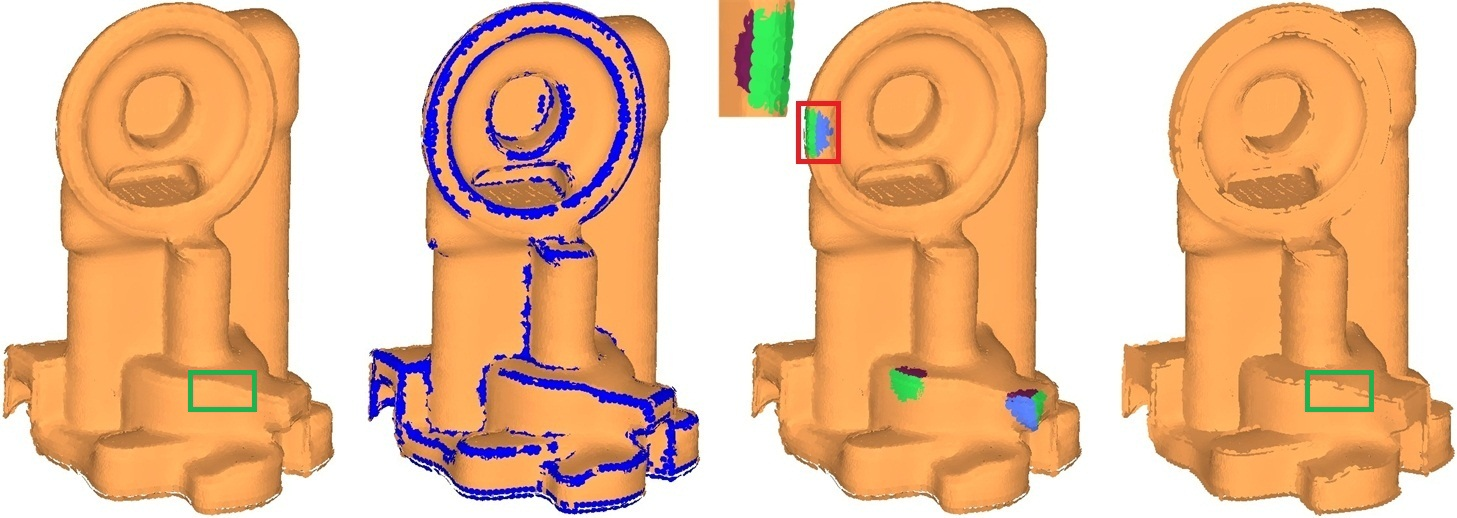
\includegraphics[width=0.8\linewidth]{oilpump_zj}\\
  \hspace{3 mm} (a) \hspace{28 mm} (b) \hspace{28 mm} (c)\hspace{28 mm} (d)
  \caption{Method overview.
         (a)Original model of oilpump. (b) Initial detected candidate feature points. (c)The classified subneighborhoods. (d)Estimated normals. }\label{fig:flow_chart}
\end{figure*}
With a noisy point cloud $\mathcal{P}=\{p_{i}\}_{i=1}^{N}$ as input, our algorithm takes three steps to estimate the normals preserving sharp features. First, we detect the points which are near the sharp features. Then, the neighborhoods of these points are segmented by their position and structure. Finally, using the results of segmentation we can select an anisotropic neighborhood to estimate the normal. The overall procedure of our method is shown in Fig. \ref{fig:flow_chart}.

\textbf{Candidate Feature Points Selection.} Normal estimation is challenging in the presence of sharp features. Hence we begin our method with a selection of points which are near sharp features and name them as \emph{candidate feature point}. Using covariance analysis of local neighborhoods, a weight is assigned to each vertex, which measures the likelihood of a vertex belongs to features. Candidate feature point are extracted by eliminating the vertex with low salience weight.
%We define the threshold automatically. First, we compute
%a histogram capturing the distribution of the weight $w$. Then the
%threshold is defined as the horizontal ordinate where the frequency
%begins to have a slow decrease.

\textbf{Subneighborhood Segmentation.} When the point is near sharp features, a neighborhood including distance smooth patches is likely to be got. We perform subspace clustering inside
the neighborhood of every candidate feature point to identify these patches. All the points in a single cluster represent a smooth region. To robustly segment these intersecting patches, we
propose a novel subspace clustering method based on structural low
rank presentation guided by credible regions. Our scheme improve the clustering results by taking both the local information and subspace structure into consideration.

\textbf{Normal Estimation} The actual normal estimation applied to a point is
chosen according to the category of the point.  If a point is not belong to the candidate feature points, the whole neighborhood is used to estimate the normal of the point. Otherwise, we choose the nearest cluster generated by subneighborhood segmentation to estimate the normal. 
\section{Low-rank subspace clustering with prior knowledge}
\label{sec:lowrank}
In this section, we present our low-rank subspace clustering framework with prior knowledge, based on which our normal estimation algorithm is designed (Section \ref{sec:algorithm}). First, we give a short review of subspace clustering. Subspace clustering is a fundamental problem which has numerous
applications in image processing and computer vision.
%
In practice, the data points are always drawn from a union of subspaces with lower intrinsic dimensions than the dimension of the ambient space.
The task of subspace clustering is to segment the data into multiple
low-dimensional linear subspaces.

\subsection{Sparse subspace clustering (SSC)}
\label{sec:subspacesegmentation}
The recently proposed sparse representation, low-rank representation achieves competitive results in subspace clustering~\cite{DBLP:journals/corr/abs-1010-2955,LiuLY10,DBLP:conf/cvpr/ElhamifarV09}. These methods are all based on the observation that a data vector can be represented by
the data vectors from the same subspace and their models can be summarized as follows
\begin{eqnarray}
min f(Z) & s.t. & X=XZ,
\end{eqnarray}
where $f(Z)$ is a matrix function, each column of the matrix $X$
represents a sample. The affinity matrix $S$ can be defined as
\begin{eqnarray}
S=|Z|+|Z'|. \label{eq:defineS}
\end{eqnarray}
Then the NCut method \cite{DBLP:journals/pami/ShiM00} is applied to get the
clustering result. The key of these methods is to
define an appropriate function $f$.


Sparse subspace clustering (SSC) proposed by E. Elhamifar \etal
~\cite{DBLP:conf/cvpr/ElhamifarV09} uses the 1D sparsity. It is an
effective method for the independent subspace clustering and the
model can be written as
\begin{eqnarray}
min \|Z\|_{1} & s.t. & X=XZ,diag(Z)=\textbf{0},
\end{eqnarray}
where $\|\cdot\|_{1}$ represents $l_{1}$-norm. However,
\cite{DBLP:conf/cvpr/NasihatkonH11} gives failure examples in dimensions higher than three. Moreover, SSC finds the sparsest
representation of each sample individually without global
constraints.
\subsection{Low-rank subspace clustring (LRSC)}
\label{sec:LRSC}
To capture the global structure of
the whole data, low-rank representation~\cite{DBLP:journals/corr/abs-1010-2955,LiuLY10}
considering the 2D sparsity, \ie the rank of a matrix, is presented for subspace clustering.
The model can be written as
\begin{eqnarray}
min \|Z\|_{*} & s.t. & X=XZ,
\end{eqnarray}
where $\|\cdot\|_{*}$ represents the sum of singular value. It is an effective subspace clustering algorithm that outperforms the state-of-the-art algorithms in handling corrupted data. However, when the subspaces are not independent, this method may fail.

%\jj{Zhuang can for dependent?} Thus Zhuang \etal
%~\cite{DBLP:conf/cvpr/ZhuangGLMZY12} proposed Non-Negative Low-Rank and Sparse (NNLRS) graph for semi-supervised learning, which can be written as
%\begin{eqnarray}
%min \|Z\|_{*} + \beta\|Z\|_{1} & s.t. & X=XZ,Z\geq \textbf{0},
%\label{eq:NNLRS}
%\end{eqnarray}
%where $\beta \geq 0$ is used to balance the influence of these two terms. This method considers both the sparsity and the global structure by combining 1D sparsity with 2D sparsity.

\subsection{Low-rank subspace clustering with prior knowledge (LRSCPK)}
\label{sec:LRSCPK}
To segment two or more intersection planes, an affinity matrix which is
dense between same class and sparse between different classes is preferred.
%
Thus we propose a low-rank subspace clustering framework (LRSCPK) with prior knowledge:
\begin{eqnarray}
min \|Z\|_{*} + \beta\|\mathcal {P}_{\Omega}(Z)\|_{1} & s.t. &
X=XZ.\label{eq:SSLRR}
\end{eqnarray}
where $\Omega$ is a guiding matrix and $0 \leq \Omega(i,j) \leq 1$,
$\mathcal {P}_{\Omega}$ can be seen as a mapping satisfying $\mathcal {P}_{\Omega}(Z)_{i,j} = \Omega(i,j)\times Z(i,j)$.
The guiding matrix $\Omega$ can be seen as prior knowledge. $\Omega$ has the property that the samples from the same
intra class contribute to a smaller weight while the samples from interclass contribute to a larger weight.
We note that the subspace can be clustered correctly even when $\Omega$ contains partial prior and gentle noise in our experiments.

%
In order to improve the robustness of this method, we replace the equality constraint of problem (\ref{eq:SSLRR}) with a soft constraint
\begin{small}
\begin{eqnarray}
min \|Z\|_{*} + \beta\|\mathcal {P}_{\Omega}(Z)\|_{1} +
\gamma\|E\|_{2,1} & s.t. & X=XZ+E, \label{eq:RSSLRR}
\end{eqnarray}
\end{small}
where $\beta$ and $\gamma$ are two parameters and we set them as 1 in this work, $\|\cdot\|_{2,1}$ is the $l_{2,1}$ norm and defined as the sum of $l_{2}$ norms of the columns of a matrix.
%To verify the effectiveness and robustness of the framework, a toy example is provided.

\subsubsection{A toy example}
\label{sec:toy}
A toy example is provided to verify the effectiveness and robustness of LRSCPK.
We sample $300$ points from two intersecting planes in $\mathbb{R}^{3}$, $150$ for
each plane.
%
Forty percent prior knowledge with $20\%$, $30\%$, $40\%$ errors are presented to LRSCPK.
%
Specifically, the ideal full guiding matrix $G\in \mathbb{R}^{300*300}$ has the property
that if two samples $p_{j}$ and $p_{k}$ are in the same plane, $G(j,k) = 0$,
otherwise $G(j,k) = 1$.
%
The guiding matrix $\Omega$ is generated by choosing $40\%$ elements of $G$ randomly and the other elements of $\Omega$ are all zeros. The errors are added by randomly selecting $20\%$, $30\%$, $40\%$ elements from the $40\%$ elements and switching their values, \ie from ones to zeros if they are ones originally (resp. zero to one).
%
As illustrated by~\fig~\ref{fig:improve} (a), (b) and (c), LRSC fails to segment two dependent subspaces, while LRSCPK generates faithful segmentation using partial prior knowledge even with considerable levels of errors.
Moreover, when the prior knowledge is seriously corrupted by errors, LRSCPK still provides a more qualified segmentation than LRSC, as shown in~\fig~\ref{fig:improve} (d).
\begin{figure*}[htbp]
\begin{center}
    \begin{tabular}{c}
        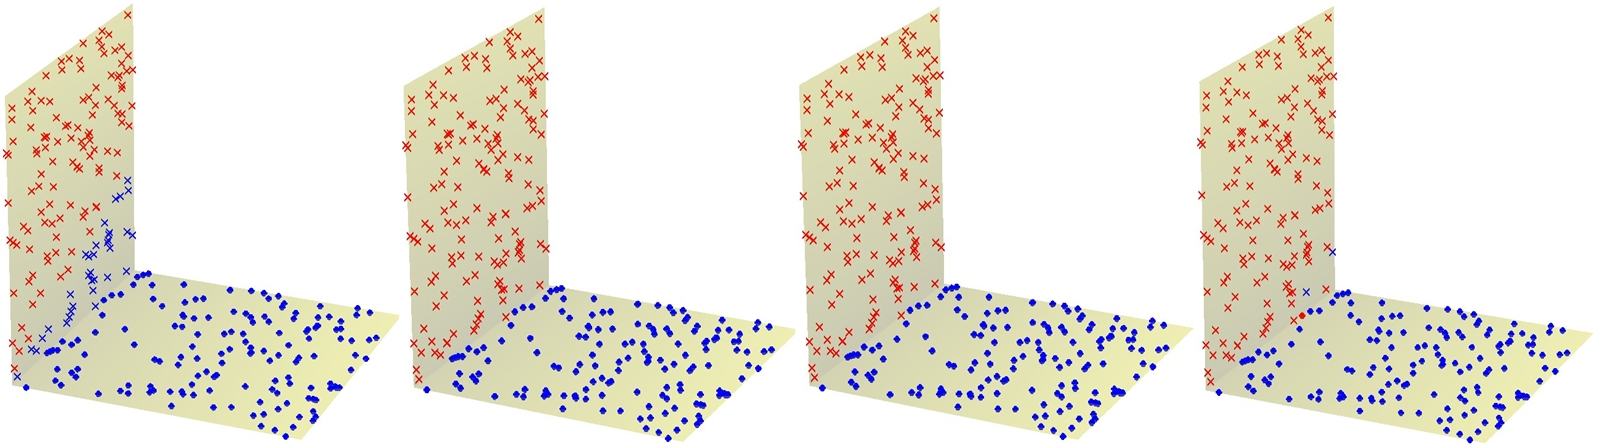
\includegraphics[width=1\linewidth]{test}\\
        \hspace{-10 mm} (a) \hspace{34 mm} (b) \hspace{34 mm} (c)\hspace{34 mm} (d)
    \end{tabular}
    \caption{Segmentation results of LRR and LRSCPK on two intersecting planes. (a) The result of LRR with $11\%$ clustering error. From (b) to (d) are the results of LRSCPK with $40\%$ prior knowledge which are corrupted by $20\%$, $30\%$ and $40\%$ errors, respectively. The clustering error is 0, 0 and $1\%$.}
    \label{fig:improve}
\end{center}
\end{figure*}

\section{LRSCPK for normal estimation}
\label{sec:algorithm}
\subsection{Overview of our algorithm}
{\label{sec:overview}}
With a noisy point cloud $\mathcal{P}=\{p_{i}\}_{i=1}^{N}$ as input, our algorithm takes three steps to estimate the normals, while preserving sharp features. First, we detect the points which are near sharp features. Then, for each of these points, the neighborhood of it is segmented by LRSCPK with prior knowledge estimated from its local structure. Finally, using the segmentation result we select a consistent subneighborhood to estimate the normal. The overall procedure of our method is shown in Fig. \ref{fig:flow_chart}.

%\textbf{Candidate feature points selection.} Normal estimation is challenging in the presence of sharp features. Hence we begin our method with a selection of points which are near sharp features and name them as \emph{candidate feature point}. Using covariance analysis of local neighborhoods, a weight is assigned to each vertex, which measures the likelihood of a vertex belongs to features. Candidate feature point are extracted by eliminating the vertex with low salience weight.
%%We define the threshold automatically. First, we compute
%%a histogram capturing the distribution of the weight $w$. Then the
%%threshold is defined as the horizontal ordinate where the frequency
%%begins to have a slow decrease.
%
%\textbf{Subneighborhood segmentation.} When the point is near sharp features, a neighborhood including distance smooth patches is likely to be got. We perform subspace clustering inside
%the neighborhood of every candidate feature point to identify these patches. All the points in a single cluster represent a smooth region. To robustly segment these intersecting patches, we
%propose a novel subspace clustering method based on structural low
%rank presentation guided by credible regions. Our scheme improve the clustering results by taking both the local information and subspace structure into consideration.
%
%\textbf{Normal estimation} The actual normal estimation applied to a point is
%chosen according to the category of the point.  If a point is not belong to the candidate feature points, the whole neighborhood is used to estimate the normal of the point. Otherwise, we choose the nearest cluster generated by subneighborhood segmentation to estimate the normal.
%As discussed earlier, we would like to identify piecewise
%smooth regions in the neighborhood of each candidate feature point before applying the normal estimation.
%The neighbourhood of each point near sharp features consists multiple smooth surface patches and each patch can be very closely approximated by a plane. Therefore the subspace clustering method proposed in the above section can be used to identify these smooth regions.

\subsection{Candidate feature points selection}
\label{subsec:candidateFeature}
Given a point $p_{i}$, we select a neighborhood $\mathcal {N}_{i}$ of size
$S$ which depends on the noise scale. Then we compute a weight
$w_{i}$ and an
estimated normal $n_{i}$ by covariance analysis of the local
neighborhood. Denote $\lambda_0 \leq \lambda_1 \leq \lambda_2$ as the singular values of the covariance matrix defined in \cite{PaulyKKG03}.
%Let $\hat{p}_{i}$ be the centroid of the local neighborhood, the
%$3\times 3$ covariance matrix $T_{i}$ of $p_{i}$ is defined as
%\begin{equation}\label{eq:pca}
%T=\frac{1}{s}\cdot\left[
%\begin{array}{c}
%p_{i1}-\hat{p}_{i}\\
%\cdots\\
%p_{is}-\hat{p}_{i}\\
%\end{array}
%\right]\cdot\left[
%\begin{array}{c}
%p_{i1}-\hat{p}_{i}\\
%\cdots\\
%p_{is}-\hat{p}_{i}\\
%\end{array}
%\right]^{T},\\
%p_{ij}\in \mathcal {N}_{i},
%\end{equation}
The weight $w_{i}$ is computed as
$$w_{i}=\frac{\lambda_{0}}{\lambda_{0}+\lambda_{1}+\lambda_{2}}.$$
%where the $\lambda_{i}$ are the eigenvalues of $T$ with $\lambda_0 \leq \lambda_1 \leq \lambda_2$.
The normal $n_{i}$ is defined as the eigenvector $v_{0}$ corresponding to the smallest eigenvalue $\lambda_{0}$.

The weight $w_{i}$ measures the confidence of $p_{i}$ belonging to a feature.
If $w_{i}$ is larger than a given threshold $w_{t}$ then $p_{i}$ is regarded as a candidate feature point.
%
Denote the distribution of $\{ w_{i} \}_{i=1}^{N}$ as $f_{w}$ and smooth it by
$$min_{\hat{f}_{w}} \quad \|\hat{f}_{w}-f_{w}\|_{F}+\|Df_{w}\|_{1},$$where $D$ is the second difference matrix, $\|\cdot\|_{F}$ and $\|\cdot\|_{1}$ represent $l_{2}$ norm and $l_{1}$ norm, respectively. We choose the $w_{t}$ after the first peak of the smoothed distribution with gently decrease, as shown in \fig \ref{fig:Candidate_threshold}.
%We choose the $w_{t}$ after the first peak of the $l_{1}$-smoothed distribution of $\{ w_{i} \}_{i=1}^{N}$ with gently decrease, as show in \fig \ref{fig:Candidate_threshold}.
\begin{figure}
  \centering
  % Requires \usepackage{graphicx}
  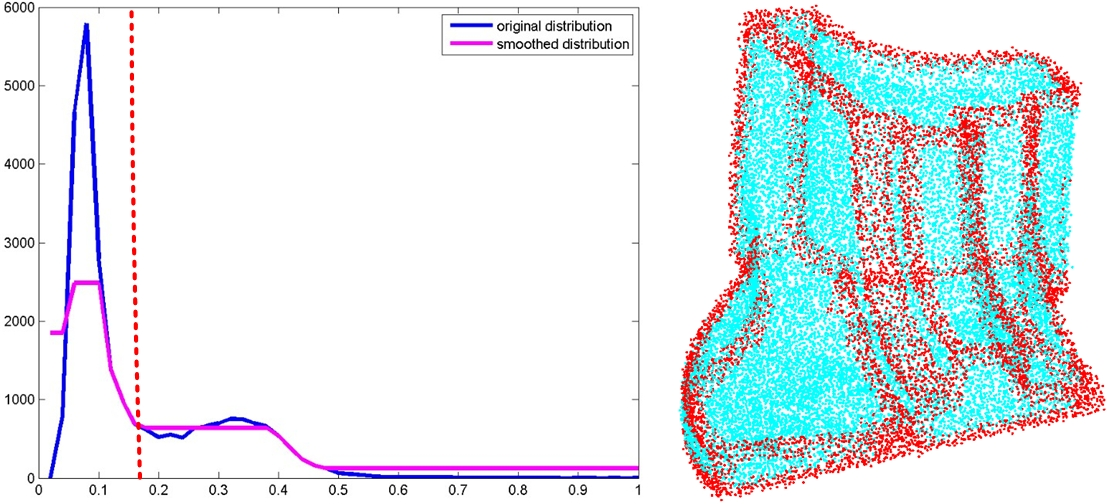
\includegraphics[width=1\linewidth]{feature}
  \caption{The choice of $w_{t}$ (left) and the candidate feature points (right). The red dashed line represent where the threshold is selected }\label{fig:Candidate_threshold}
\end{figure}

\subsection{Subneighborhood segmentation}
\label{sec:Subneighborhood_Segmentation}
\subsubsection{Subneighborhood segmentation by subspace clustering}
For a candidate feature point $p_{i}$, we first select a larger neighborhood $\mathcal {N}_{i}^{*}$ of size $S^{*}$ than $\mathcal{N}_{i}$ used for candidate feature points selection, \ie $S^{*}>S$.
In the local coordinates with $p_{i}$ as the origin, the neighbor point $p_{ij}$ of $p_{i}$ is represented as
$p_{ij} = [x_{j}, y_{j}, z_{j}, n_{xj}, n_{yj}, n_{zj}]',j = 1, \ldots, S^{*},$ where
$[x_{j},y_{j},z_{j}]$ is the coordinate of $p_{ij}\in\mathcal{N}_{i}^{*}$ and
$[n_{xj}, n_{yj}, n_{zj}]$ is its normal computed by PCA.
The sampling matrix is defined as $X = [p_{i1}, p_{i2}, \ldots, p_{iS^{*}}]$.
The optimal coefficient matrix $Z\in \mathbb{R}^{S^{*}\times S^{*}}$ can be computed by solving~\eq~(\ref{eq:RSSLRR}).
After obtaining the affinity matrix from ~\eq~(\ref{eq:defineS}), we segment $\mathcal {N}_{i}^{*}$ by NCut. Since the number of subspaces is unknown, we segment these neighbor points into two classes first.
If any one of them is not a subspace, it is segmented into two classes further.
The iterative progress is terminated until each class is a subspace.

Determining whether or not a class is a subspace is performed by fitting a plane to the class and measuring the average residual.
If the average residual is smaller than a threshold $\tau_{f}$, the class is determined as a subspace.
To automatically compute an appropriate $\tau_{f}$, we compute normalized average residual histograms of candidate feature points and non-candidate points respectively and set $\tau_{f}$ as the horizontal ordinate
where the two histograms cross, as illustrated in \fig \ref{fig:fit_threshold}.
\begin{figure}
  \centering
  % Requires \usepackage{graphicx}
  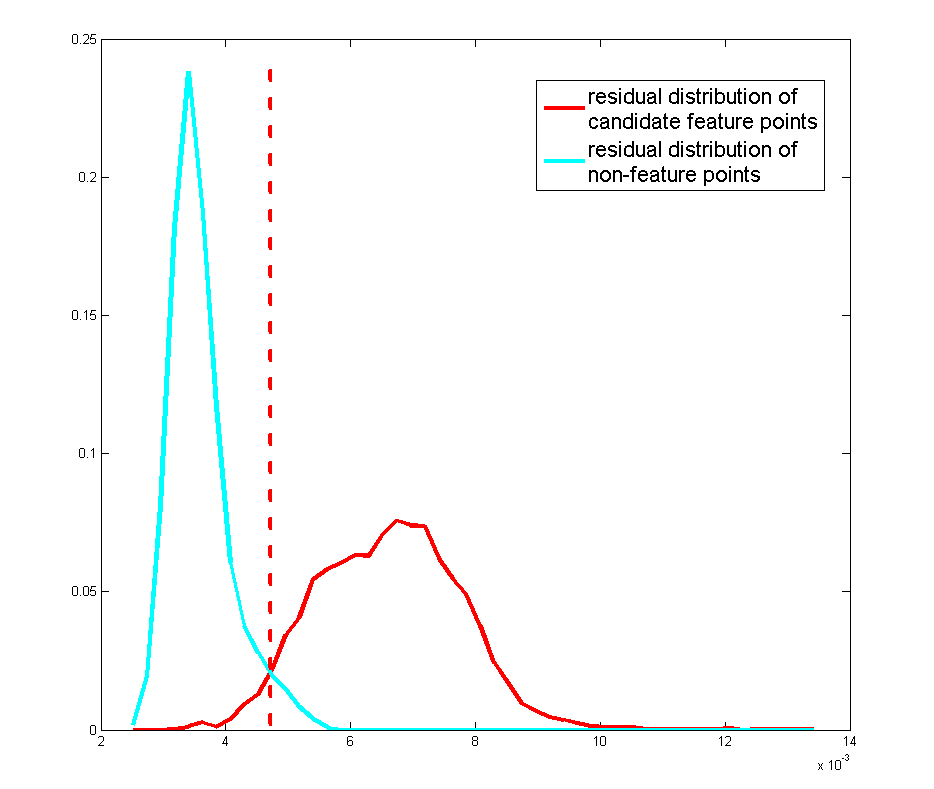
\includegraphics[width=0.9\linewidth]{fit}
  \caption{The choice of $\tau_{f}$. The red dashed line represent where the threshold is selected}\label{fig:fit_threshold}
\end{figure}

\subsubsection{Construction of the guiding matrix}
The guiding matrix $\Omega$ can be built by various ways. We estimate it according to the observation that although normals estimated by PCA are error-prone for points around sharp features, they are reliable for points away from sharp features. Thus the reliable regions are used to guide the segmentation of the neighborhood.
For any two points $p_{ij}$ and $p_{ik}$ in the neighborhood of $p_i$, we compute the normals of $p_{ij}$ and $p_{ik}$ using their $K$-nearest neighbors respectively and compute the distance $D(j,k)$ between the two planes specified by the normals.
If $p_{ij}$ or $p_{ij}$ is adjacent to sharp features, \ie with larger $w_{ij}$ or $w_{ik}$, no plane approximates its neighborhood well. We randomly choose $r$ points from its $K$-nearest neighbors to estimate its normal. The construction of the distance matrix $D$ is shown in \textbf{algorithm} \ref{CDM_pseudocode}.

%Based on the observation that when a point is far from sharp
%features the point and its neighbors often belong to the same
%subspace, we can fit a subspace $\hat{\mathcal {S}}$ by using the
%point and its $K$-nearest neighbors. If two points $j$ and $k$ lie in the same
%subspace $\mathcal {S}_{i}$, their locally estimated subspaces
%$\hat{\mathcal {S}}_{j}$ and $\hat{\mathcal {S}}_{k}$ should be the
%same, while if the two points lie in different subspaces,
%$\hat{\mathcal {S}}_{j}$ and $\hat{\mathcal {S}}_{k}$ should be
%different. Therefore, we can use the distance between $\hat{\mathcal
%{S}}_{j}$ and $\hat{\mathcal {S}}_{k}$ to define a distance matrix
%$D$. However, when the point adjacent to sharp features, the point
%and its neighbors may not belong to the same subspace. Hence, we can
%not directly use the point and its neighbors to fit the subspace.
%Actually there should be some of the neighbors belonging to the same
%subspace with the current point. Therefore we randomly choose $r$
%points from its $K$-nearest neighbors to fit a subspace. The process of constructing
%distance matrix is shown in \textbf{algorithm} \ref{CDM_pseudocode}.
\begin{algorithm}[t]
\linesnumbered \KwIn{\emph{CandidateFeaturePointSet} $A$,
\emph{Non-FeaturePointSet} $B$;} \KwOut{\emph{DistanceMatrix}$D$;}
\BlankLine

\emph{DistanceMatrix} $D=\textbf{0}$;\\
\For{each point $p_{ij} \in A \cup B$} {
    \For{each point $p_{ik} \in A \cup B$}
    {
    \If{$p_{ij} \not\in A $ }
    {
     Normal $n1$ = normal(NearestNeighbors);
     }
    \Else
    {
     Normal $n1$ = normal(RandomNearestNeighbors);
    }
    \If{$p_{ik} \not\in A $ }
    {
     Normal $n2$ = normal(NearestNeighbors);
     }
    \Else
    {
     Normal $n2$ = normal(RandomNearestNeighbors);
    }
    $D(j,k) = 1 - |<n1,n2>|$
    }
}  \caption{Construct The Distance Matrix} \label{CDM_pseudocode}
\end{algorithm}

$D(j,k)$ can be seen as the probability of
points $j$ and $k$ belonging to different planes,~\ie subspaces.
We set $\Omega(j,k) = 1$ if $D(j,k)$ is larger than a threshold $\tau_{max}$, and set $\Omega(j,k) = 0$ otherwise.
%
Denoting $D_{max}$ as the set of the largest $40\%$ elements in the
matrix $D$, we set $\tau_{max} = min(D_{max},1-cos(45^{\circ}))$.
This setting of $\tau_{max}$ means that when the angle between the two estimated planes of $p_{ij}$ and $p_{ik}$ is larger than $45^{\circ}$, they are predicted to belong to different subspaces.

\textbf{Sequence of computing the guiding matrix.}
In order to improve the reliability of the guiding matrix, we first segment neighborhoods of points with smaller $w_i$,
store the segmentation results of each neighborhood and use them to update the guiding matrices of points around sharp features which are computed later.
We denote the number of $p_{ij}$ and $p_{ik}$ in the same
subspace and in different subspaces as $R_{jk}$ and $N_{jk}$, respectively.
If $R_{jk}>N_{jk}$, we define $\Omega(j,k)$ as $\Omega(j,k) = min\left ( \Omega(j,k), 1- \frac{R_{jk}}{R_{jk}+N_{jk}}\times exp(-1/R_{jk}) \right )$.
Otherwise we define $\Omega(j,k)$ as $\Omega(j,k) =
max\left ( \Omega(j,k),\frac{N_{jk}}{R_{jk}+N_{jk}}\times exp(-1/N_{jk}) \right )$.

\textbf{Improvement for points near sharp features.}
When $p_{ij}$ or $p_{ik}$ is near sharp features, the normal estimated using $r$ random points from a point's $K$-nearest neighbors is not reliable.
Therefore the reliability of the probabilities $D(j,:)$ or $D(k,:)$ is lower.
We reduce the corresponding element in the guiding matrix $\Omega$.
Specifically, if only one of $p_{ij}$ or $p_{ik}$ is around sharp features we set $\Omega(j,k) = \alpha \Omega(j,k),$ $0<\alpha<1$.
If both of them are near sharp features we set $\Omega(j,k) = \beta \Omega(j,k),$ $0< \beta < \alpha$.
%
We take $\alpha = 0.6$ and $\beta = 0.2$ in our experiments.
%\begin{algorithm}
%\linesnumbered \KwIn{\emph{CandidateFeaturePointSet} $A$,
%\emph{Non-FeaturePointSet} $B$,\emph{DistanceMatrix} $D$;}
%\KwOut{\emph{GuidingMatrix}$\Omega$;} \BlankLine
%
%\emph{GuidingMatrix} $\Omega=\textbf{0}$;\\
%\For{each point $p_i \in A \cup B$} {
%    \For{each point $p_j \in A \cup B$}
%    {
%    \If{$D(i,j) > threshold$ }
%    {
%      \If{$p_i \not\in A$ and $p_j \not\in A$}
%      {
%      $L(i,j) = 1$
%      }
%      \If{$p_i \in A$ and $p_j \in A$}
%      {
%      $L(i,j) = \alpha$
%      }
%      \If{($p_i \not\in A$ and $p_j \in A$) or ($p_i \in A$ and $p_j \not\in A)$}
%      {
%      $L(i,j) = \beta$
%      }
%    }
%    }
%}  \caption{Construct The Leading Matrix} \label{CLM_pseudocode}
%\end{algorithm}

\subsection{Normal estimation}
For the non-candidate points, their neighborhood is isotropic and normals estimated by PCA is used. For any candidate feature point $p_i$, its neighborhood is anisotropic. We segment its neighborhood into several isotropic subneighborhoods by the method described in section \ref{sec:Subneighborhood_Segmentation}.
For each subneighborhood, a plane is fitted to $p_i$ and the subneighborhood.
Thus each subneighborhood has a fitting residual. The subneighborhood with the minimum residual is identified as a consistent subneighborhood of $p_i$. Then an accurate normal can be easily estimated using the consistent subneighborhood.

%Denoting $n$ as the number of points and $n_{f}$ as the number of candidate feature points, the complexity of our method, RNE and HF are $O(n\mathrm{log}n + n_{f}\times s^{*3})$, $O(n\mathrm{log}n)$ and $O(n\mathrm{log}n)$, respectively.
\subsection{Time complexity of our algorithm}
\label{sec:timing}
Our algorithm takes three steps: candidate feature points selection, subneighborhood segmentation and normal estimation. The time complexity of them are $O(N\mathrm{log}N)$, $O(N_{f}\times(\mathrm{log}N + (S^{*})^{3}))$ and $O(N_{f}\mathrm{log}N)$, respectively, where $N$ is the number of points and $N_{f}$ is the number of the candidate feature points.
%-
We use Kd-tree for neighborhood search (the $\mathrm{log}N$ factor) and repeat some local operations for each point (the N factor) in the first step and for each candidate feature point (the $N_{f}$ factor) in the remaining steps.
%-
For each candidate feature point, the most time-consuming operation is to solve ~\eq~(\ref{eq:RSSLRR}) when segmenting  subneighborhood of size $S^{*}$. A modified alternating direction method (ADM) is designed with the same complexity of the standard one \cite{convergence} (the $(S^{*})^{3}$ factor) and presented in Appendix 1.
%
Thus the time complexity of our algorithm is $O(N\mathrm{log}N + N_{f}\times (S^{*})^{3})$.
%{\color{blue}The complexity of solving ~\eq~(\ref{eq:RSSLRR}) can be reduced to $O((S^{*})^{2})$ using the linearized alternating direction approach \cite{LinLS11}.} \jz{The parallel computing can be employed further to speed up our algorithm.(could delete)}

\section{Results and applications}
\label{sec:results}
A variety of noisy point clouds with sharp features are tested to evaluate the performance of our approach.
We also compare our method with some classic and state-of-the-art algorithms: PCA \cite{DBLP:conf/siggraph/HoppeDDMS92}, robust normal estimation (RNE) \cite{DBLP:journals/cg/LiSKCDJ10} and hough transform (HF) \cite{DBLP:journals/cgf/BoulchM12}.


To evaluate the estimation accuracy, the Root Mean Square measure with threshold ($RMS\_\tau $) \cite{DBLP:journals/cgf/BoulchM12} is used as follows:
\begin{equation}\label{eq:NEE}
RMS\_\tau = \sqrt{\frac{1}{|\mathcal{P}|}\sum_{p\in \mathcal{P}}(f(\widehat{n_{p,ref}n_{p,est}}))^{2}},
\end{equation}
where
$$f(\widehat{n_{p,ref}n_{p,est}})=\left \{
\begin{array}{rl}
    \widehat{n_{p,ref}n_{p,est}}, \quad & if\widehat{n_{p,ref}n_{p,est}}<\tau \\
    \pi /2,\quad & otherwise \\
\end{array}
\right. ,
$$
$n_{p,ref}$ is the reference normal at $p$ and $n_{p,est}$  is the
estimated one.
%
We take $\tau = 10$ degrees, as proposed by \cite{DBLP:journals/cgf/BoulchM12}. In the following, the points with the measure greater than $10$ degrees are considered as bad points.

%%%%%%%%%%%%%%%%%%%%%%%%%%%%%%%%%%%%%%%%%%%%%%%%%%%%%%%%%%%%%%%%%%%%%%%%%%%%%%%%%%%%%%%%%%%%%%%%%%%%%%%%%%%%
%%%%%%%%%%%%%%%%%%%%%%%%%%%%%%%%%%%%%%%%%%%%%%%%%%%%%%%%%%%%%%%%%%%%%%%%%%%%%%%%%%%%%%%%%%%%%%%%%%%%%%%%%%%%
The parameters $S$, $S^{*}$, $K$ and $r$ of our algorithm are chosen as $S=70$, $S^{*}=120$, $K=30$ and $r=10$ for all models in this section.
%
We use the same neighborhood size $S^{*}$ for all the three methods.
All other parameters, if any, are set to default.
%
We evaluate the estimation accuracy on the data with synthetic noise: a centered Gaussian noise with deviation defined as a percentage of average distance between points.
%We evaluate precision and speed on data with artificial noise: a centered Gaussian noise with deviation defined as a percentage of the diagonal of the axis-aligned bounding box.

\subsection{Comparisons with other methods}

\textbf{Sharp features with shallow angles.} In \fig~\ref{fig:octahedron_03_result}, we compare the normal estimation results of the Octahedron model. It contains sharp features generated by two intersection planes with shallow angles. Normals estimated by PCA are overly smoothed on/near sharp features. Those of HF are also a bit smooth, since normals produced by triples sampled from different sides are likely to vote for the same bin when the angle is shallow.
%
The bottom row of \fig~\ref{fig:octahedron_03_result} demonstrates that our algorithm  preserves sharp features better. We can see that the number of bad points and $RMS\_\tau$ are both smaller from our method, as shown in the middle row of \fig~\ref{fig:octahedron_03_result} and \tab \ref{tab:Computational_Statistics}.

\begin{figure}
\begin{center}
    \begin{tabular}{c}
        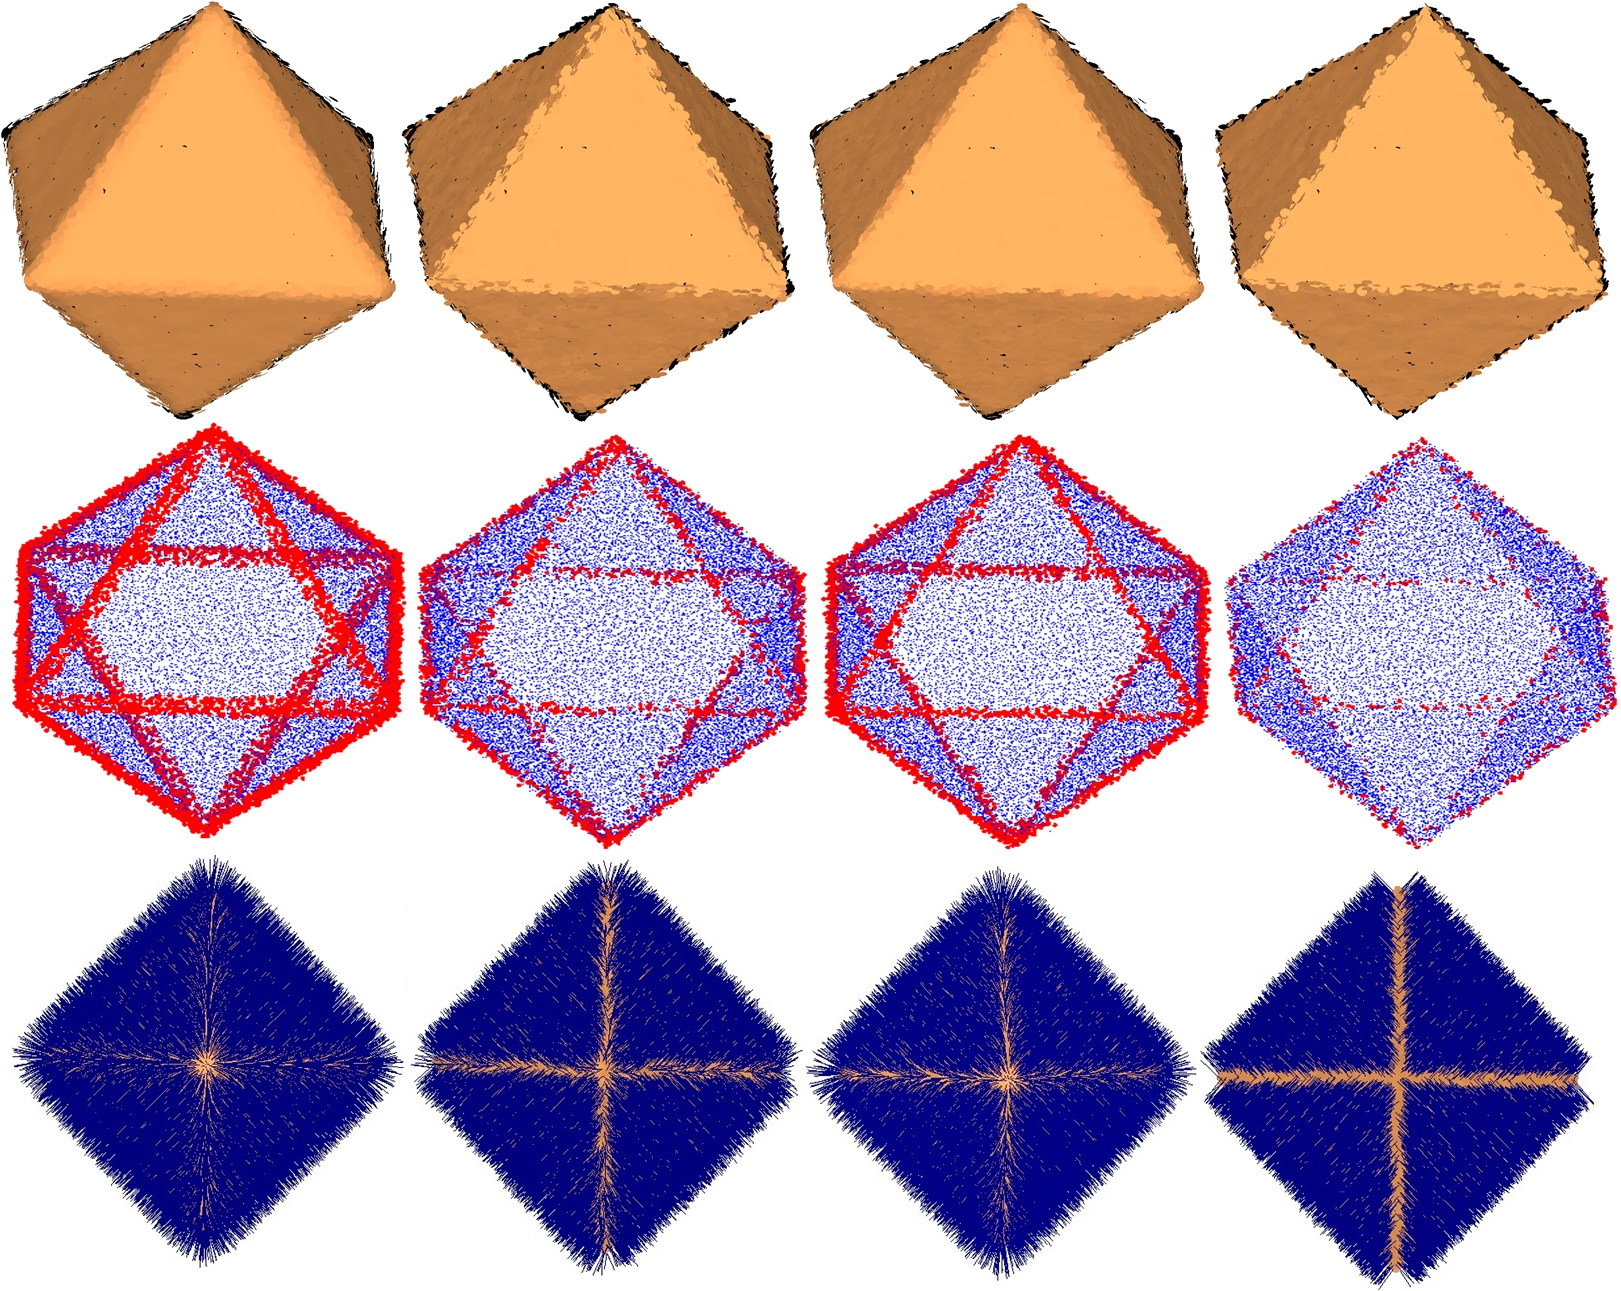
\includegraphics[width=1\linewidth]{oc}
    \end{tabular}
    \caption{Comparison for Octahedron model with $50\%$ noise.  From the top to bottom row are the results rendering using surfels, the visualization of bad points and top view of the generated normals, respectively. Left to right are the results of PCA, RNE, HF and our algorithm, respectively.\label{fig:octahedron_03_result}}
\end{center}
\end{figure}

\textbf{Neighborhood with multiple features.} The normal estimation results of Fandisk model are compared in \fig~\ref{fig:fandisk_01_result}.
%
The neighborhood of a point may contain multiple feature lines as the marked narrow-band regions in \fig~\ref{fig:fandisk_01_result}.
The complex neighborhood structure brings more challenges to the existing normal estimation methods.
%
As \fig~\ref{fig:fandisk_01_result} shown, PCA, RNE and HF generate more bad points around the narrow-band regions.
%
Our method utilizing the neighborhood's structure information does not have this flaw.
%
In addition, the bottom row of \fig~\ref{fig:fandisk_01_result} shows that our method preserves shape features comparatively better in presence of noise, while the others all blur sharp features.
%
%The bad points number and $RMS\_\tau$ listed in \tab \ref{tab:Computational_Statistics} provide further evidence to show the advantage of our method.



The bad point distributions of PCA, RNE, HF and our method are presented in \fig~\ref{fig:histogram} for the Octahedron and Fandisk models. We notice that the number of bad points from our method are much less than other methods in all normal deviation regions from 10 to 90 degree nearly.
%
For the Fandisk model, PCA obtains the smallest number of bad points with normal deviation between 80 to 90 degrees among all compared methods. It is because that the normals near sharp features by PCA are excessively smoothed and the largest deviations are almost 40 to 60 degrees.
%
%Based on the similar derivation, HF introduces a bit smoothness near sharp features and leads to less normal deviation between 70 to 90 degree.
%
The higher deviation between the above regions from RNE, HF and our method is mainly because that heavy noise makes the intersection of two planes becoming a ribbon from a line, where the points are supposed to have two directions.

\begin{figure*}[htbp]
\begin{center}
    \begin{tabular}{c}
        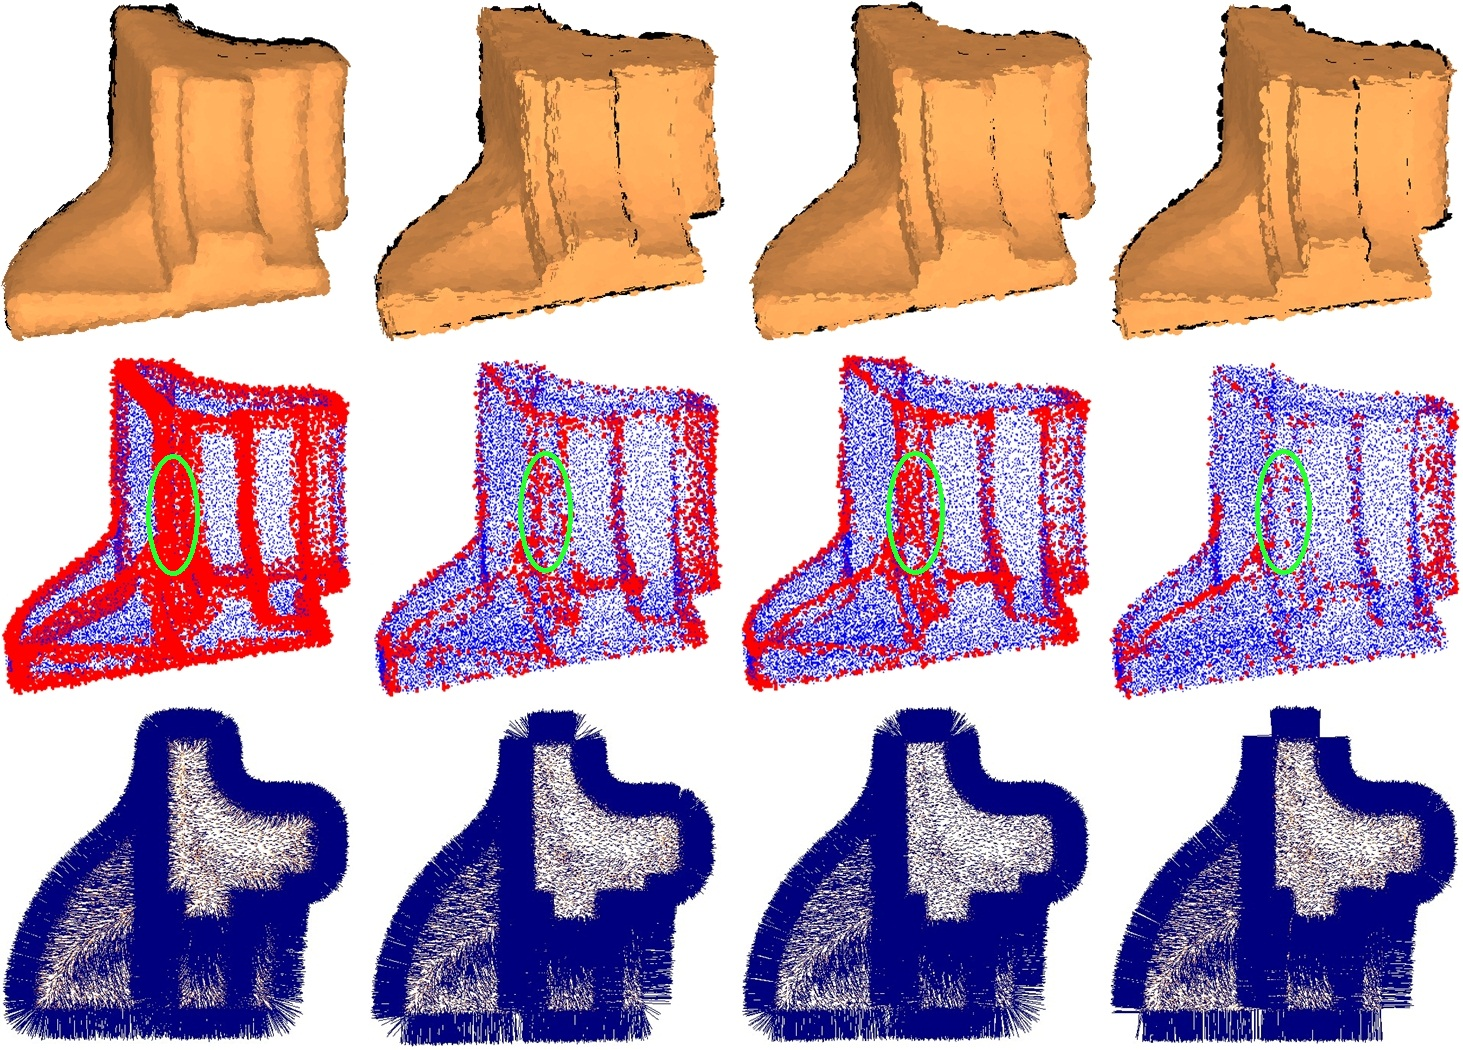
\includegraphics[width=0.8\linewidth]{fandisk_mark}\\
    \end{tabular}
    \caption{Comparison for Fandisk model with $50\%$ noise. From top to bottom row are the results rendering using surfels, the visualization of bad points and top view of the generated normals, respectively. Left to right are the results of PCA, RNE, HF and our algorithm, respectively.\label{fig:fandisk_01_result}}
\end{center}
\end{figure*}

\begin{figure*}[htbp]
\begin{center}
    \begin{tabular}{c c}
        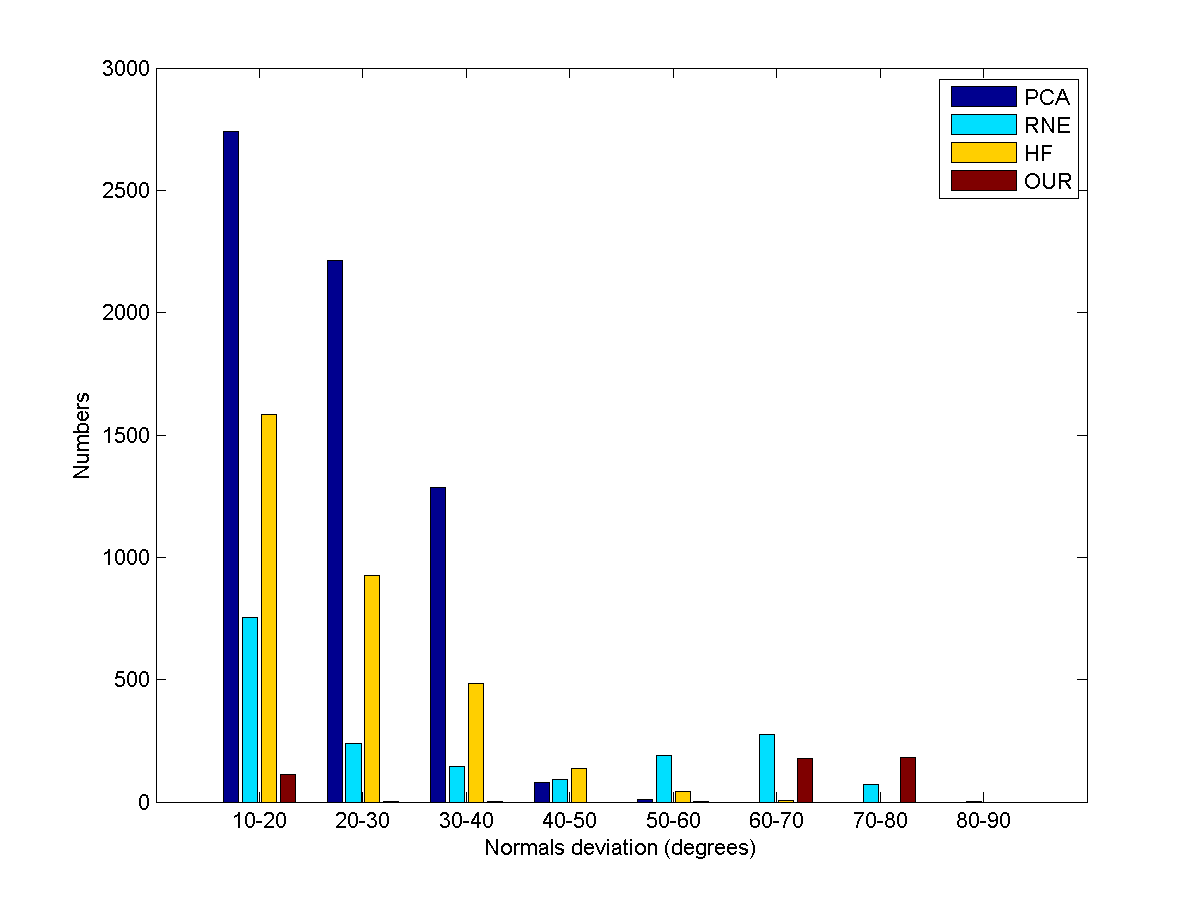
\includegraphics[width=0.5\linewidth]{octahedron_03_histogram} &
        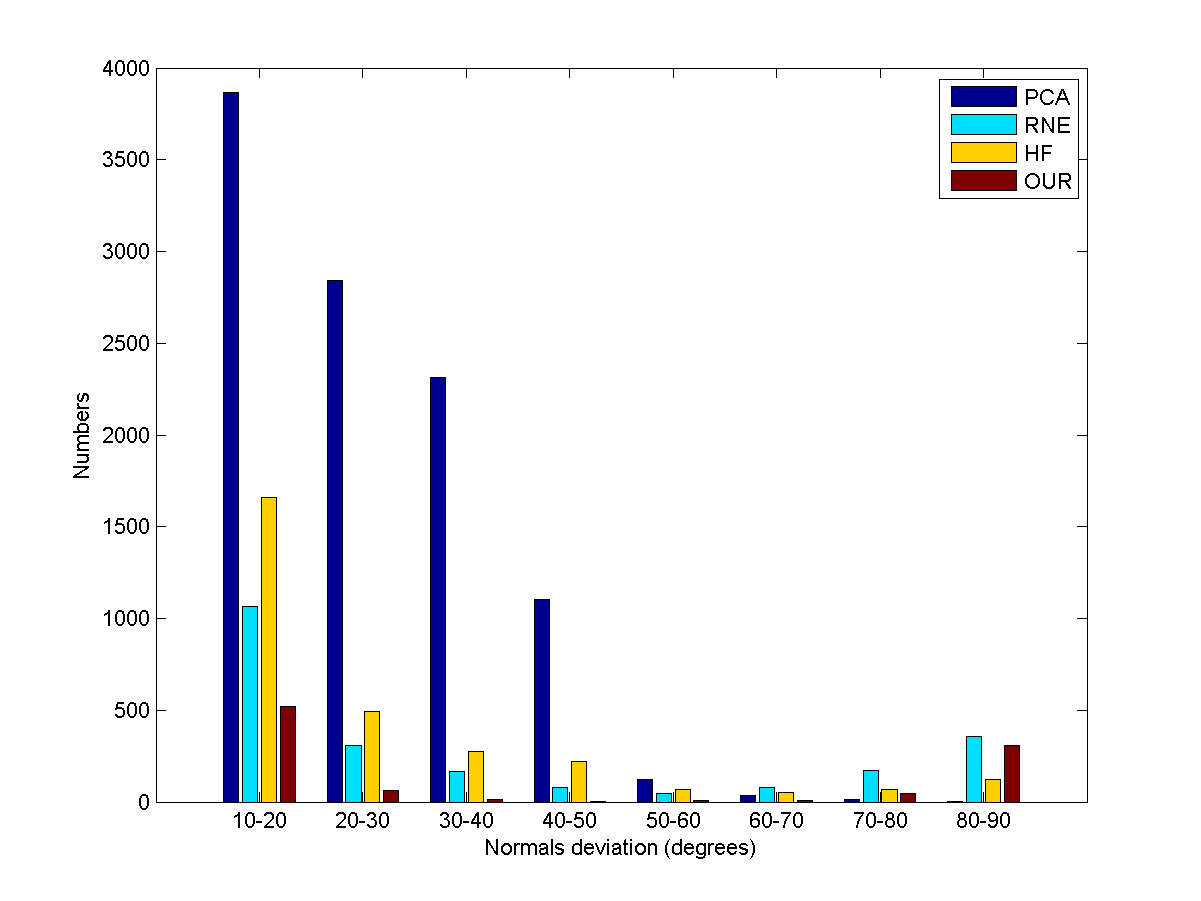
\includegraphics[width=0.5\linewidth]{fandisk_t1_histogram}
    \end{tabular}
    \caption{The histograms of the normal deviation on Octahedron model (left) and Fandisk model (right) shown in \fig \ref{fig:octahedron_03_result} and \fig \ref{fig:fandisk_01_result}, respectively.\label{fig:histogram}}
\end{center}
\end{figure*}

\textbf{Variational density near sharp features.}
Fig. \ref{fig:cube_02_result}  shows the normals estimated on a Cube sampled with face-specific
variations of density. PCA and RNE are severely affected by the non-uniform sampling. Since HF has designed a sampling strategy to deal with density variation, it performs better than PCA and RNE. However, there are still some errors near sharp features. Our method can effectively overcome the sampling anisotropy around sharp features.

%\begin{figure}[htbp]
%\begin{center}
%    \begin{tabular}{c}
%        \includegraphics[width=1\linewidth]{cube_t2_results}\\
%        \includegraphics[width=1\linewidth]{cube_t2_errs}
%    \end{tabular}
%    \caption{Results of Cube model with $50\%$ noise. Top is the estimated normals and bottom is the visualization of bad points. Left to right are the estimated results of PCA, RNE, HF and our algorithm, respectively.\label{fig:cube_02_result}}
%\end{center}
%\end{figure}
\begin{figure}[htbp]
\begin{center}
    \begin{tabular}{c c c c}
        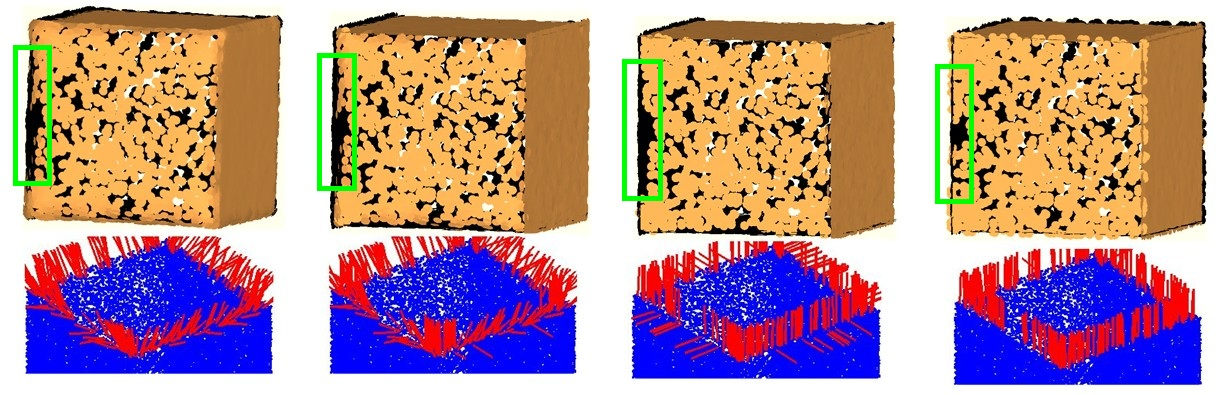
\includegraphics[width=1\linewidth]{cube}
    \end{tabular}
    \caption{Comparison for Cube model with $50\%$ noise. Density is uniform on each face; if density is 1 for the front face, then it is 5 for the upper face and 10 for the right face. The top row contains the results rendering using surfels, and the bottom row contains the top view of computed normals of the front face of the Cube model.  Left to right are the results of PCA, RNE, HF and our algorithm, respectively. \label{fig:cube_02_result}}
\end{center}
\end{figure}

\textbf{Computational statistics.}
To evaluate our method more precisely, models with different noise scales are computed, and $RMS\_\tau$ and the number of bad points are presented in Tab. \ref{tab:Computational_Statistics}. The statistics show that our method achieves the lowest $RMS\_\tau$ and NBP. More accurate normals are estimated under different noise scales.

\begin{table*}
\centering
\caption{\label{tab:Computational_Statistics}$RMS\_\tau$ and the number of bad points (NBP) on Fandisk, Octahedron  and Cube model with different noise scales.}
\begin{tabular}{|c|c|c|c|c|c|c|c|c|c|}
\hline
\multirow{2}{*}{Model} & \multirow{2}{*}{Noise scale} & \multicolumn{2}{|c}{PCA} & \multicolumn{2}{|c}{RNE} & \multicolumn{2}{|c}{HF} & \multicolumn{2}{|c|}{OUR} \\
\cline{3-10}
  & & $RMS\_\tau$ & NBP & $RMS\_\tau $ & NBP & $RMS\_\tau $ & NBP & $RMS\_\tau $ & NBP\\
\hline \hline
 Octahedron & $40\%$ & 0.7730 & 6338 & 0.3115 & 1005 & 0.4399 & 2034 & \textbf{0.1424} & \textbf{200} \\
 Octahedron & $50\%$ & 0.7722 & 6324 & 0.4123 & 1772 & 0.5496 & 3183 & \textbf{0.2174} & \textbf{478} \\
 Octahedron & $60\%$ & 0.7773 & 6406 & 0.4910 & 2518 & 0.6161 & 4002& \textbf{0.2986} & \textbf{914} \\
 Fandisk & $40\%$ & 0.9874 & 10206 & 0.3708 & 1469 & 0.4022 & 1668 & \textbf{0.2601} & \textbf{688} \\
 Fandisk & $50\%$ & 0.9921 & 10303 & 0.4694 & 2272 & 0.5341 & 2957 & \textbf{0.3088} & \textbf{970} \\
 Fandisk & $60\%$ & 1.0010 & 10487 & 0.5578 & 3214 & 0.6568 & 4485 & \textbf{0.3809} & \textbf{1483} \\
 Cube & $40\%$ & 0.5889 & 4510 & 0.2606 & 879 & 0.1043 & 135 & \textbf{0.0667} & \textbf{51} \\
 Cube & $50\%$ & 0.5865 & 4473 & 0.2537 & 829 & 0.1063 & 138 & \textbf{0.0674} & \textbf{50} \\
 Cube & $60\%$ & 0.5864 & 4471 & 0.2577 & 851 & 0.1147 & 159 & \textbf{0.0851} & \textbf{82} \\
\hline
\end{tabular}
\end{table*}

\subsection{More results for raw scans of real objects}
\label{sec:moreResults}
We also apply our method to real scanned point clouds, see~\fig~\ref{fig:realObjects} and~\fig~\ref{fig:shutter}, in which the typical imperfections, such as noise, outliers and non-uniform distribution are ubiquitous.
%-demonstrate the efficacy of our algorithm.
Although the edges of these models are corrupted with noise, especially for the Genus2 and Box models in ~\fig~\ref{fig:realObjects}, our algorithm recovers them faithfully.
%-
The Genus2 model also contains close-by surface sheets in the marked regions. The normal estimation approaches based on distance, such as PCA and its variants, tend to be affected greatly, while our structure based method not.
%-
Both the Armadillon and Taichi models are non-uniform sampled. The Taichi model has complex structures in the marked region of~\fig~\ref{fig:realObjects}. Our algorithm preserves the sharp feature well even in such complicated case.
%-
Tiny structures challenge normal estimation. The Shutter in~\fig~\ref{fig:shutter} contains many such tiny structures. When some of them are sampled adequately as the marked region, faithful normals are estimated by our method and the tiny structures can be visualized clearer.

\begin{figure*}
\begin{center}
    \begin{tabular}{c}
        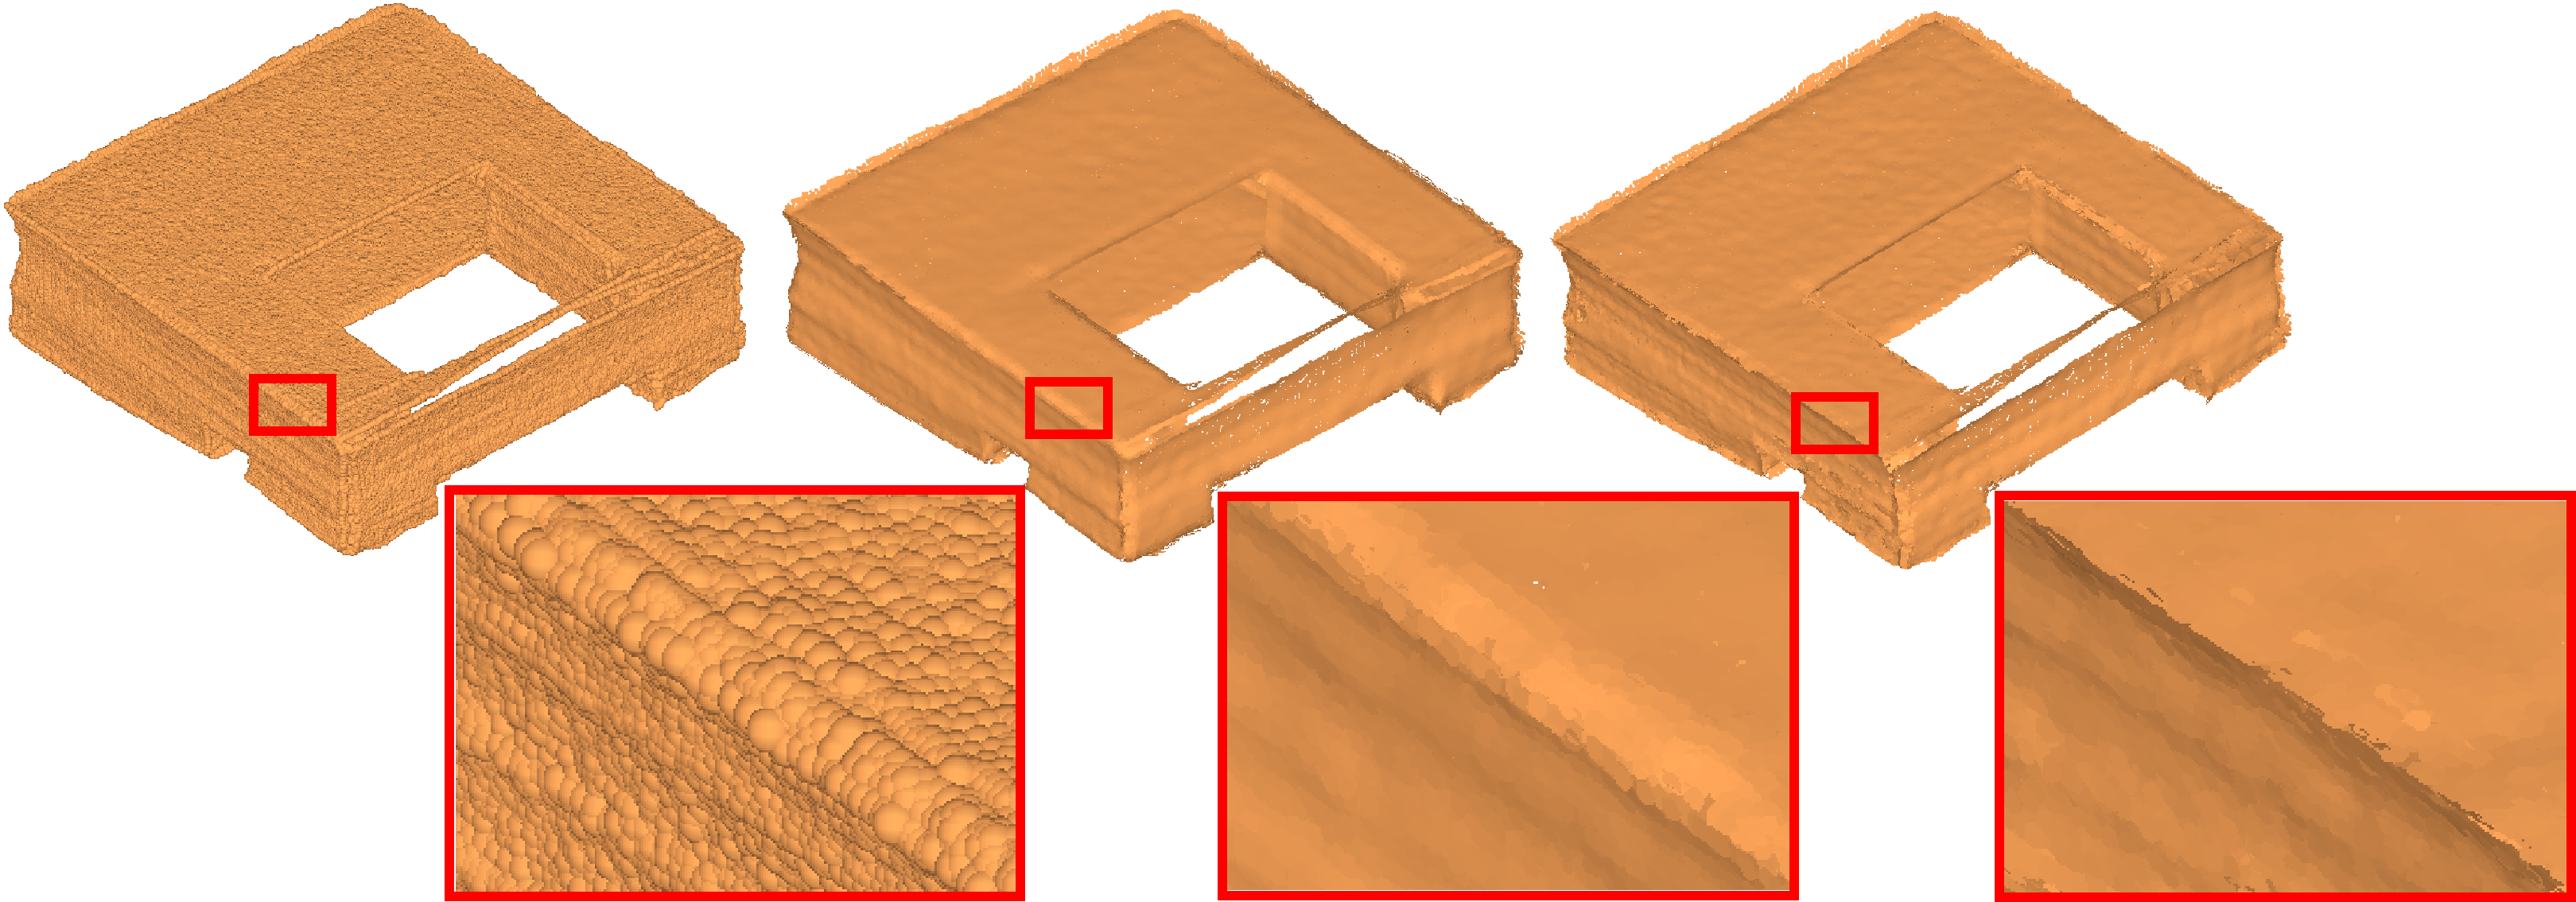
\includegraphics[width=0.8\linewidth]{box}\\
        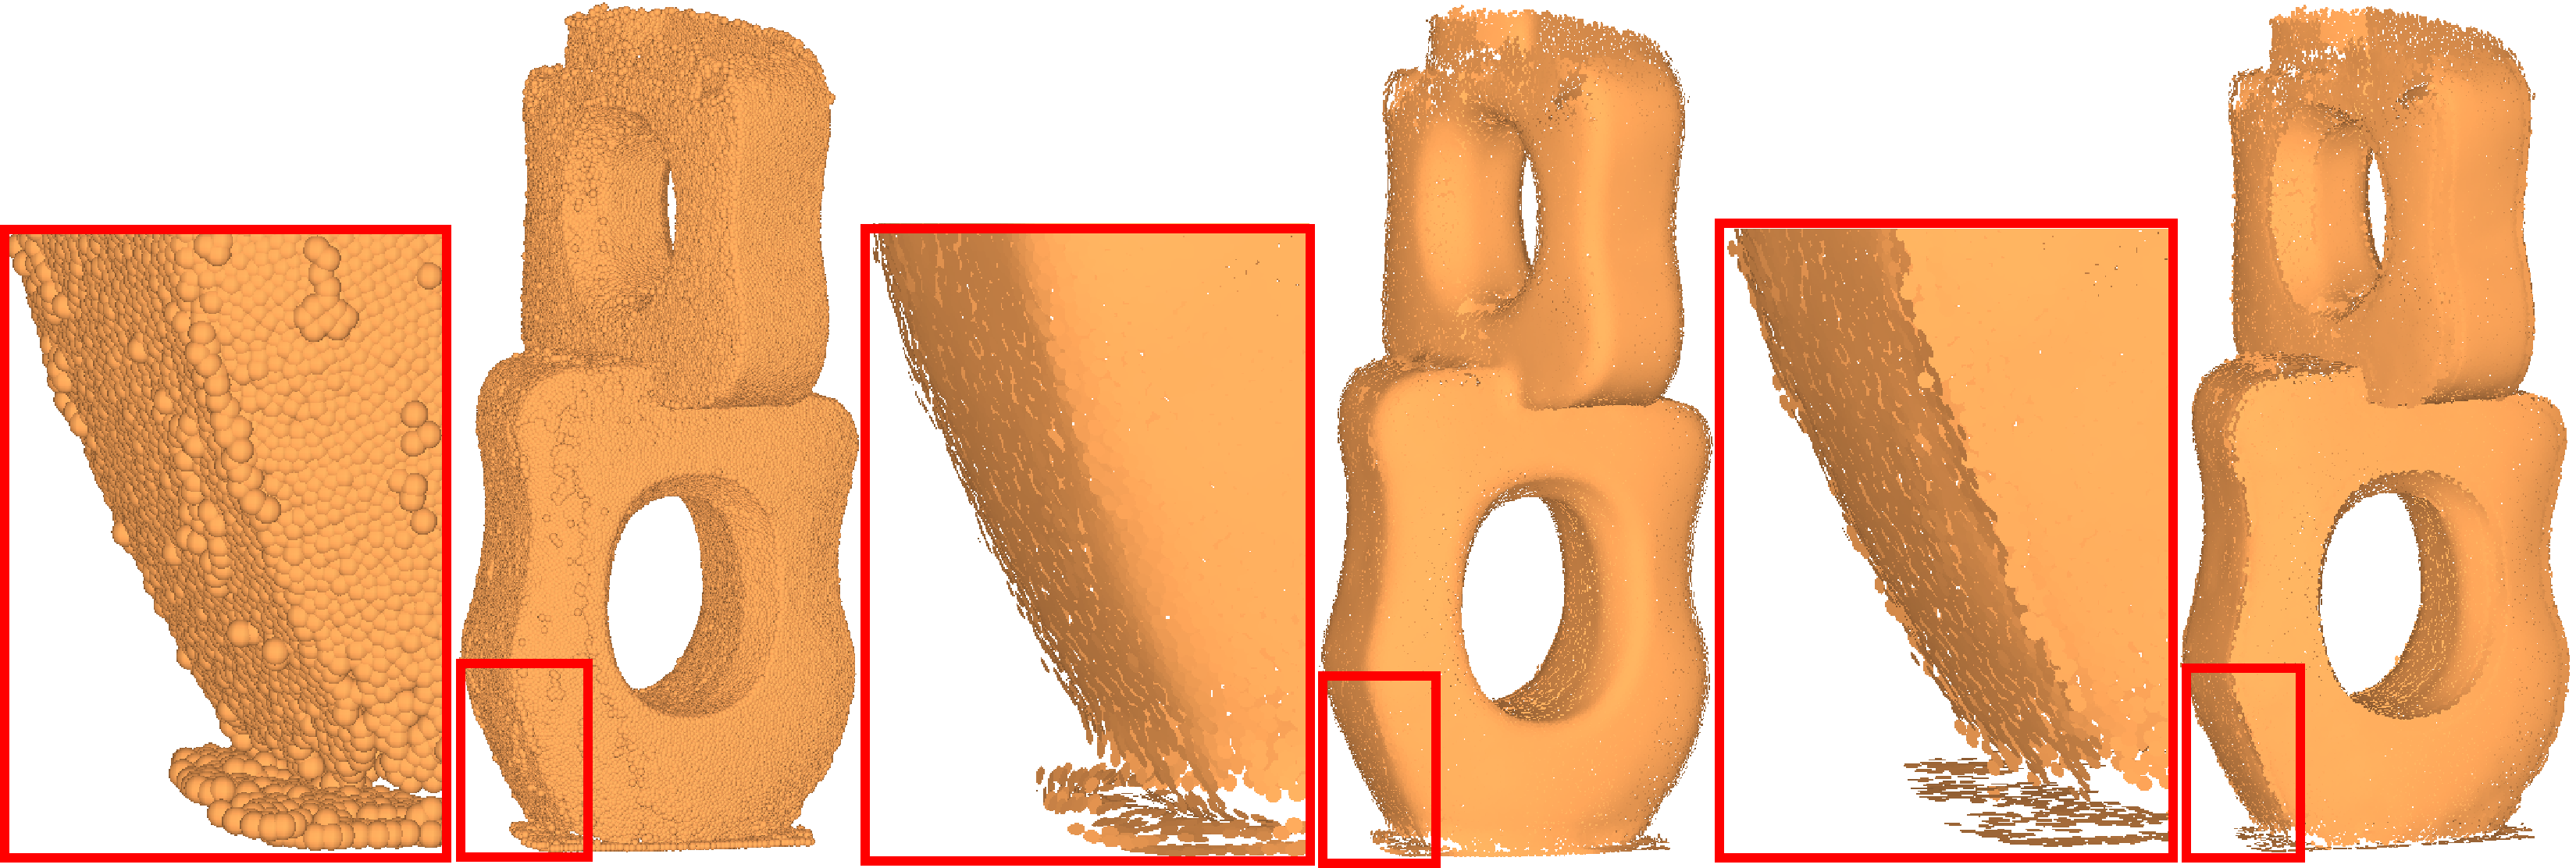
\includegraphics[width=0.8\linewidth]{geners1}\\
        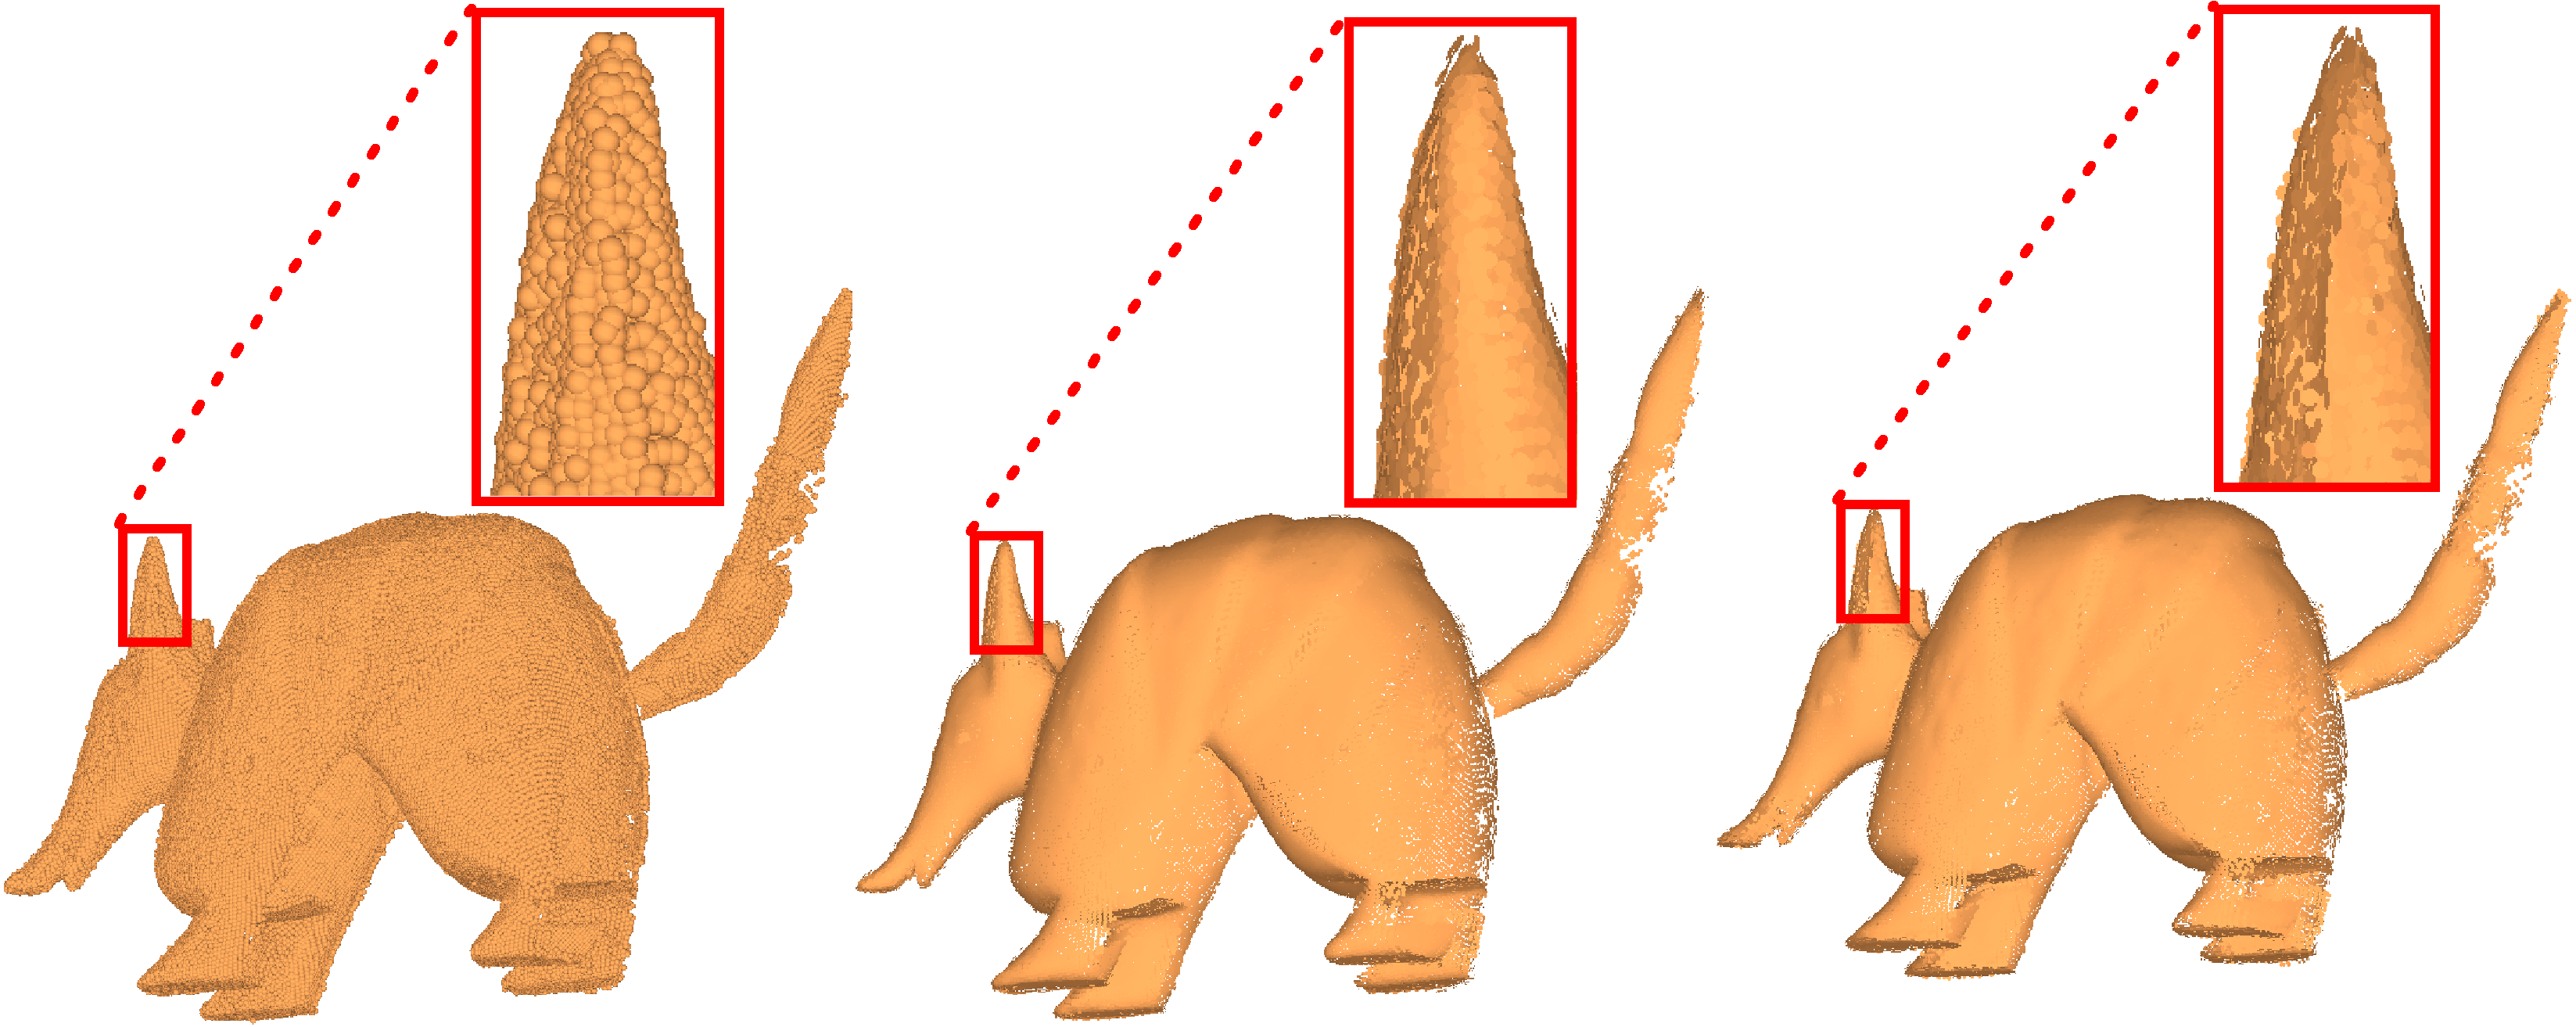
\includegraphics[width=0.8\linewidth]{armadillon}\\
        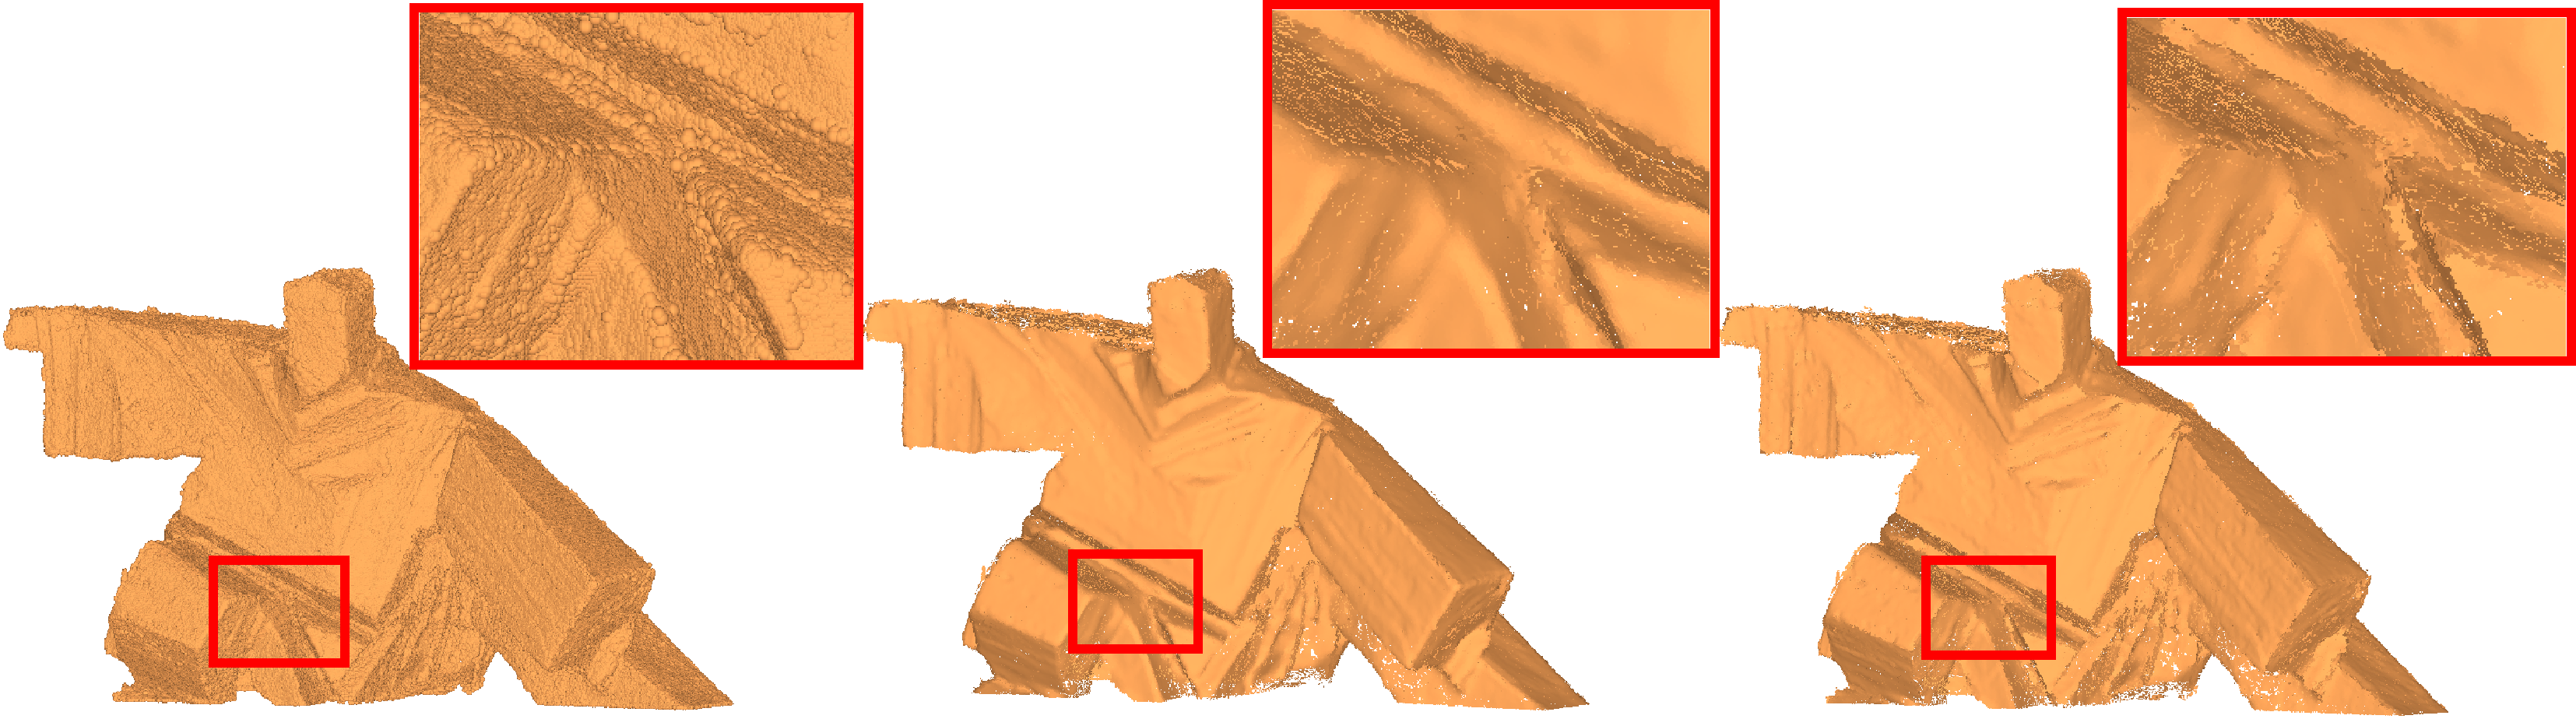
\includegraphics[width=0.8\linewidth]{taichi}\\
    \end{tabular}
    \caption{Normal estimation for raw scans of real objects: Box (222.5k points), Genus2 (50k points), Armadillon (99.4k points) and Taichi (537.6k points). Left to right are the input model, the results of PCA and our algorithm, respectively.\label{fig:realObjects}}
\end{center}
\end{figure*}

\begin{figure}
\begin{center}
    \begin{tabular}{c c }
        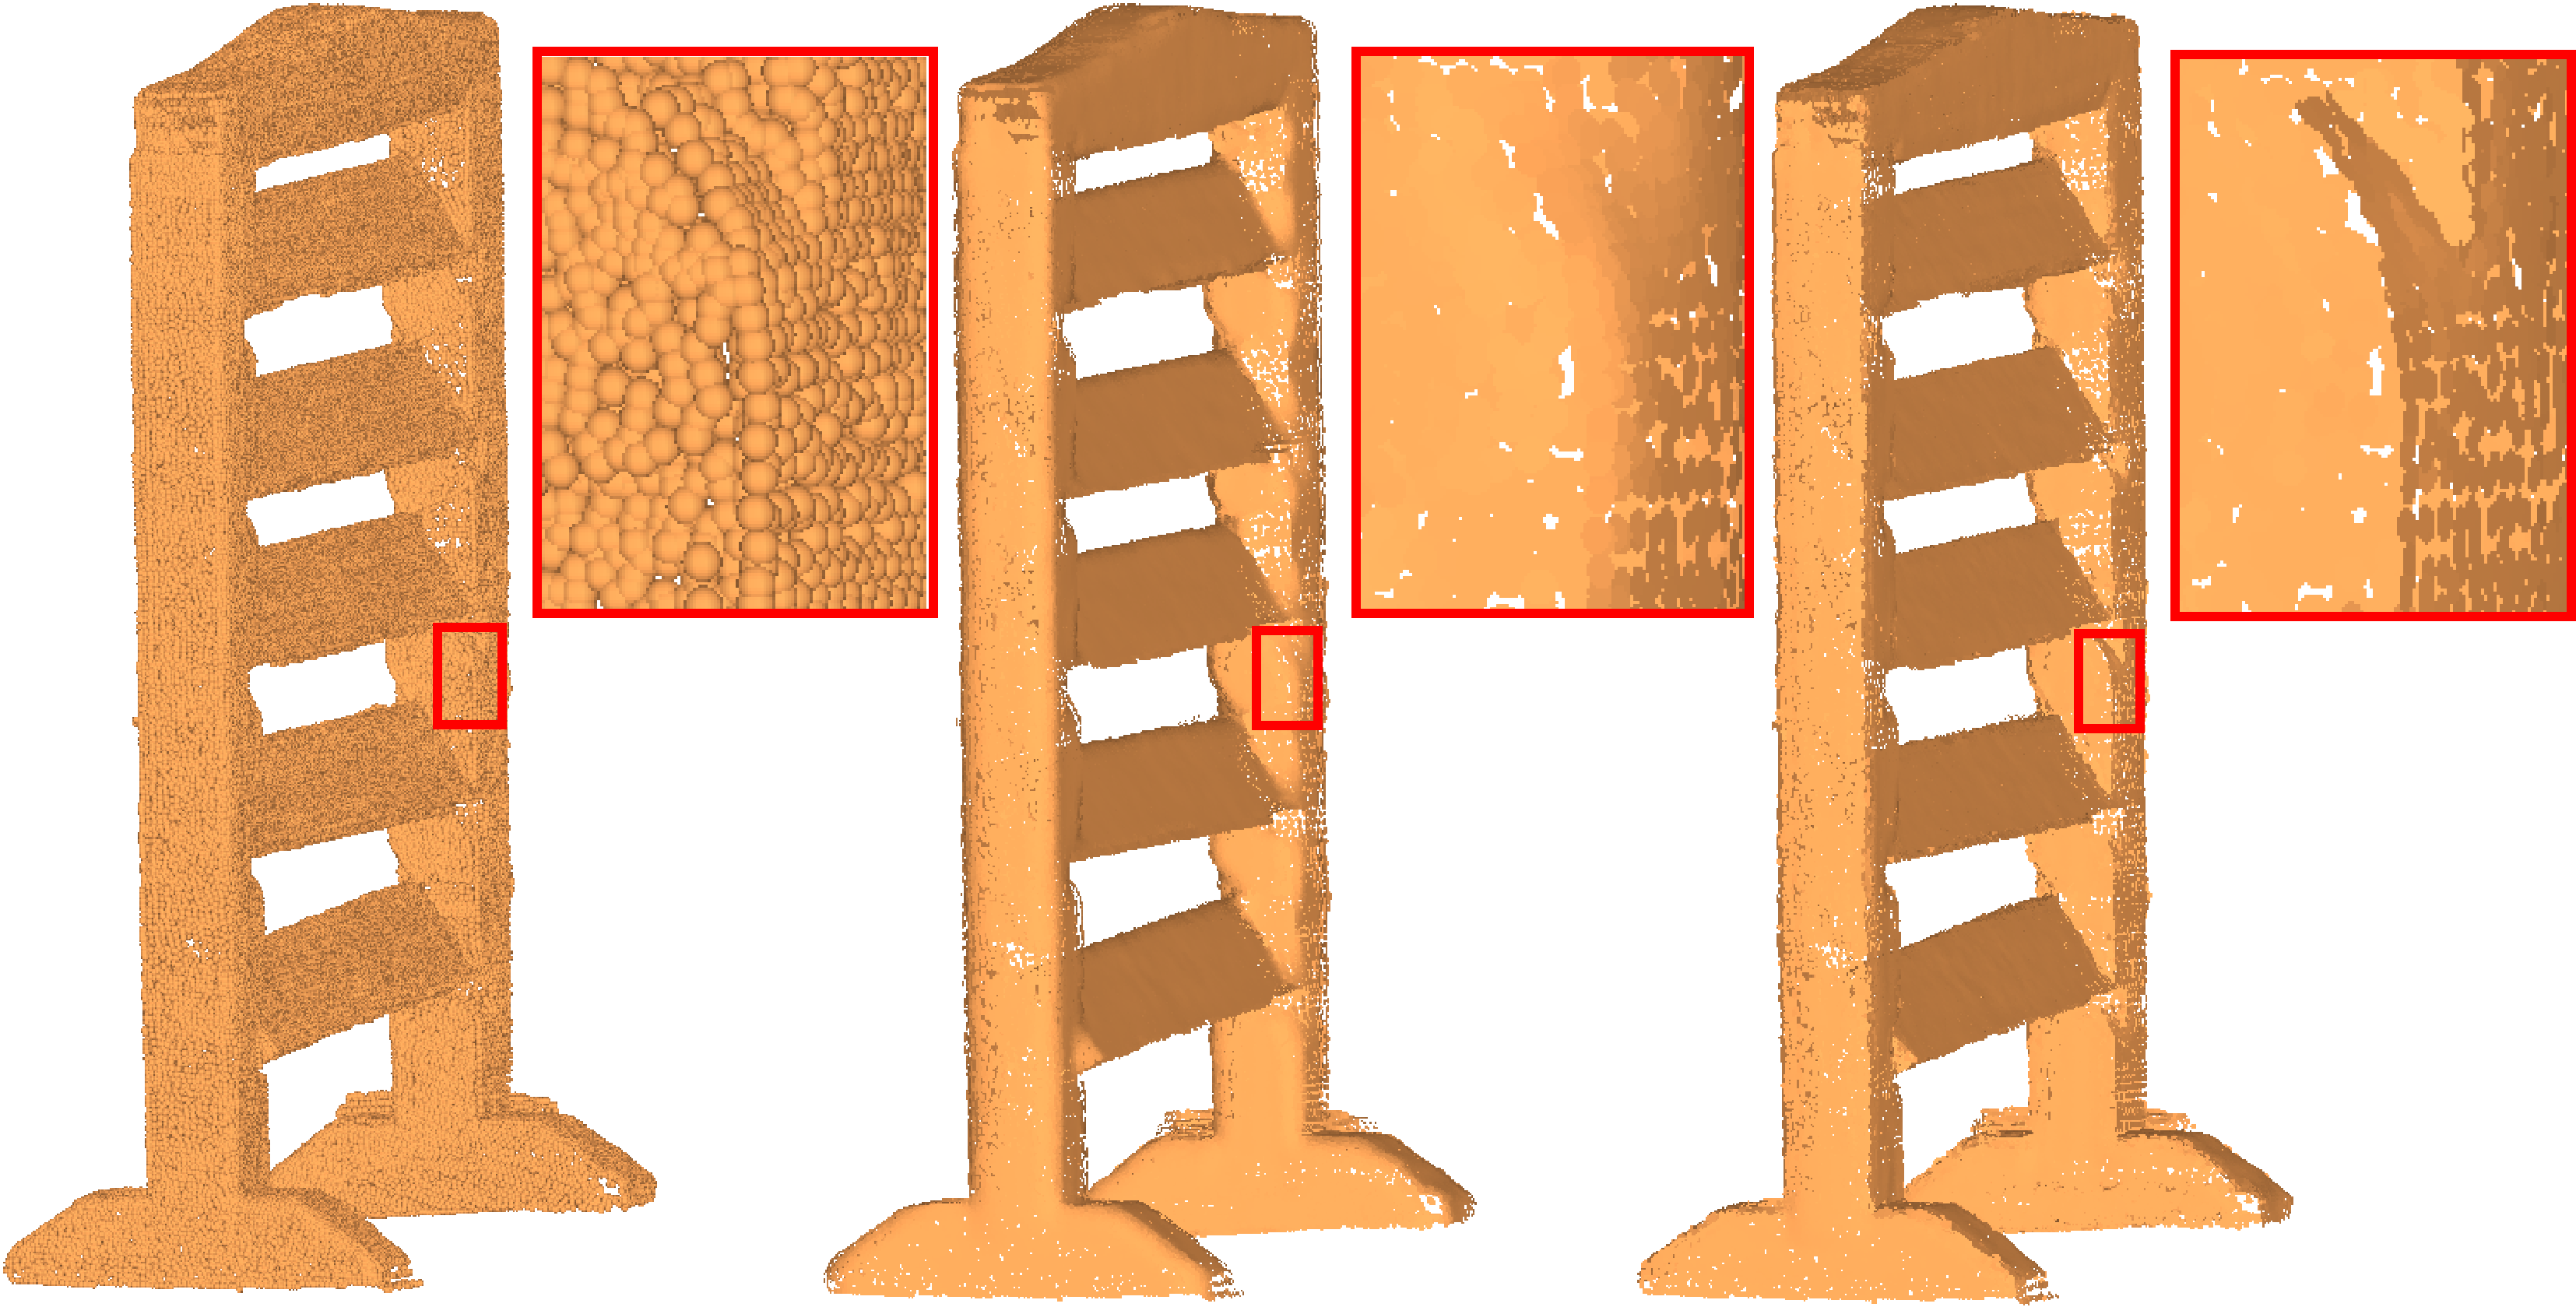
\includegraphics[width=1\linewidth]{shutter}
    \end{tabular}
    \caption{Normal estimation for the Shutter model. Left to right are the input raw scan model with 291.2k points, the results of PCA and our algorithm, respectively. \label{fig:shutter}}
\end{center}
\end{figure}
%Box (222.5k points <222481>), Genus2 (50k points <50050>), Armadillon (99.4k points <99416>) and Taichi (537.6k points <537564>), Shutter (291.2k points <291219>).
%\begin{figure*}
%\begin{center}
%    \begin{tabular}{c c }
%        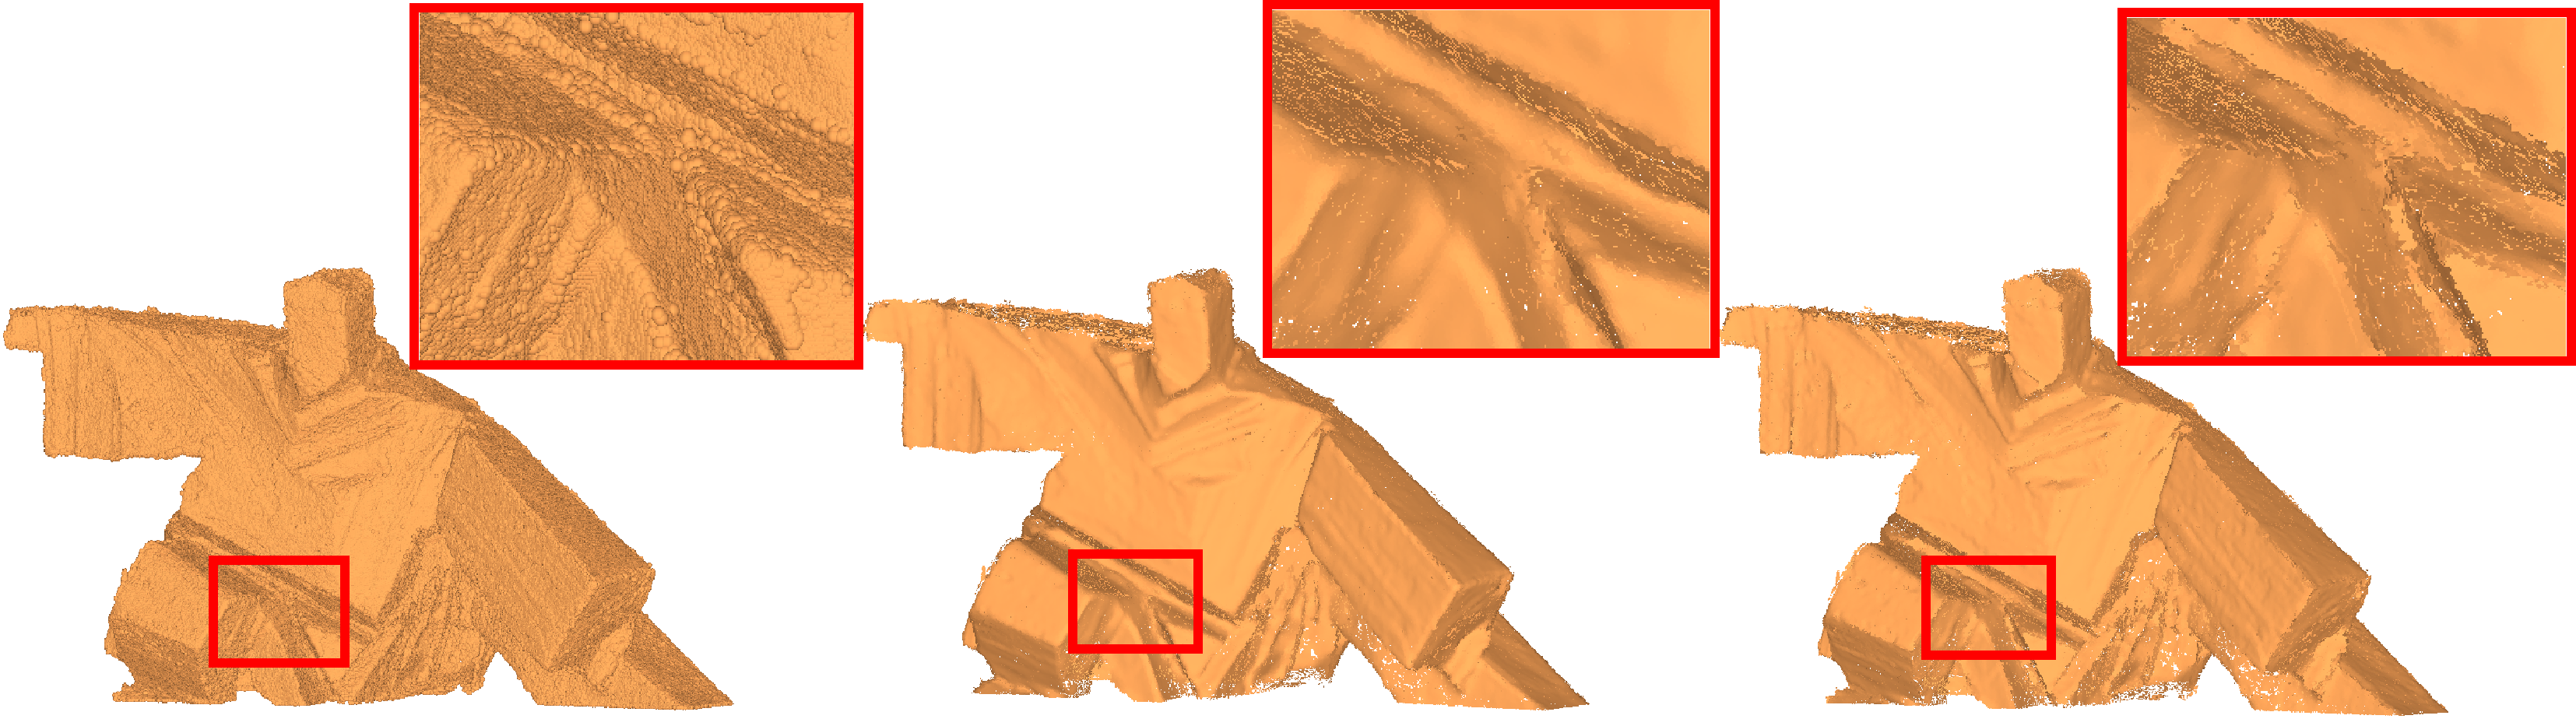
\includegraphics[width=1\linewidth]{taichi}
%    \end{tabular}
%    \caption{{\color{red}Normal estimation results for Taichi by using PCA and our algorithm. Left to
%     right are the raw scan, the results of PCA and our algorithm, respectively.}\label{fig:taichi}}
%\end{center}
%\end{figure*}
%\begin{figure*}
%\begin{center}
%    \begin{tabular}{c c }
%        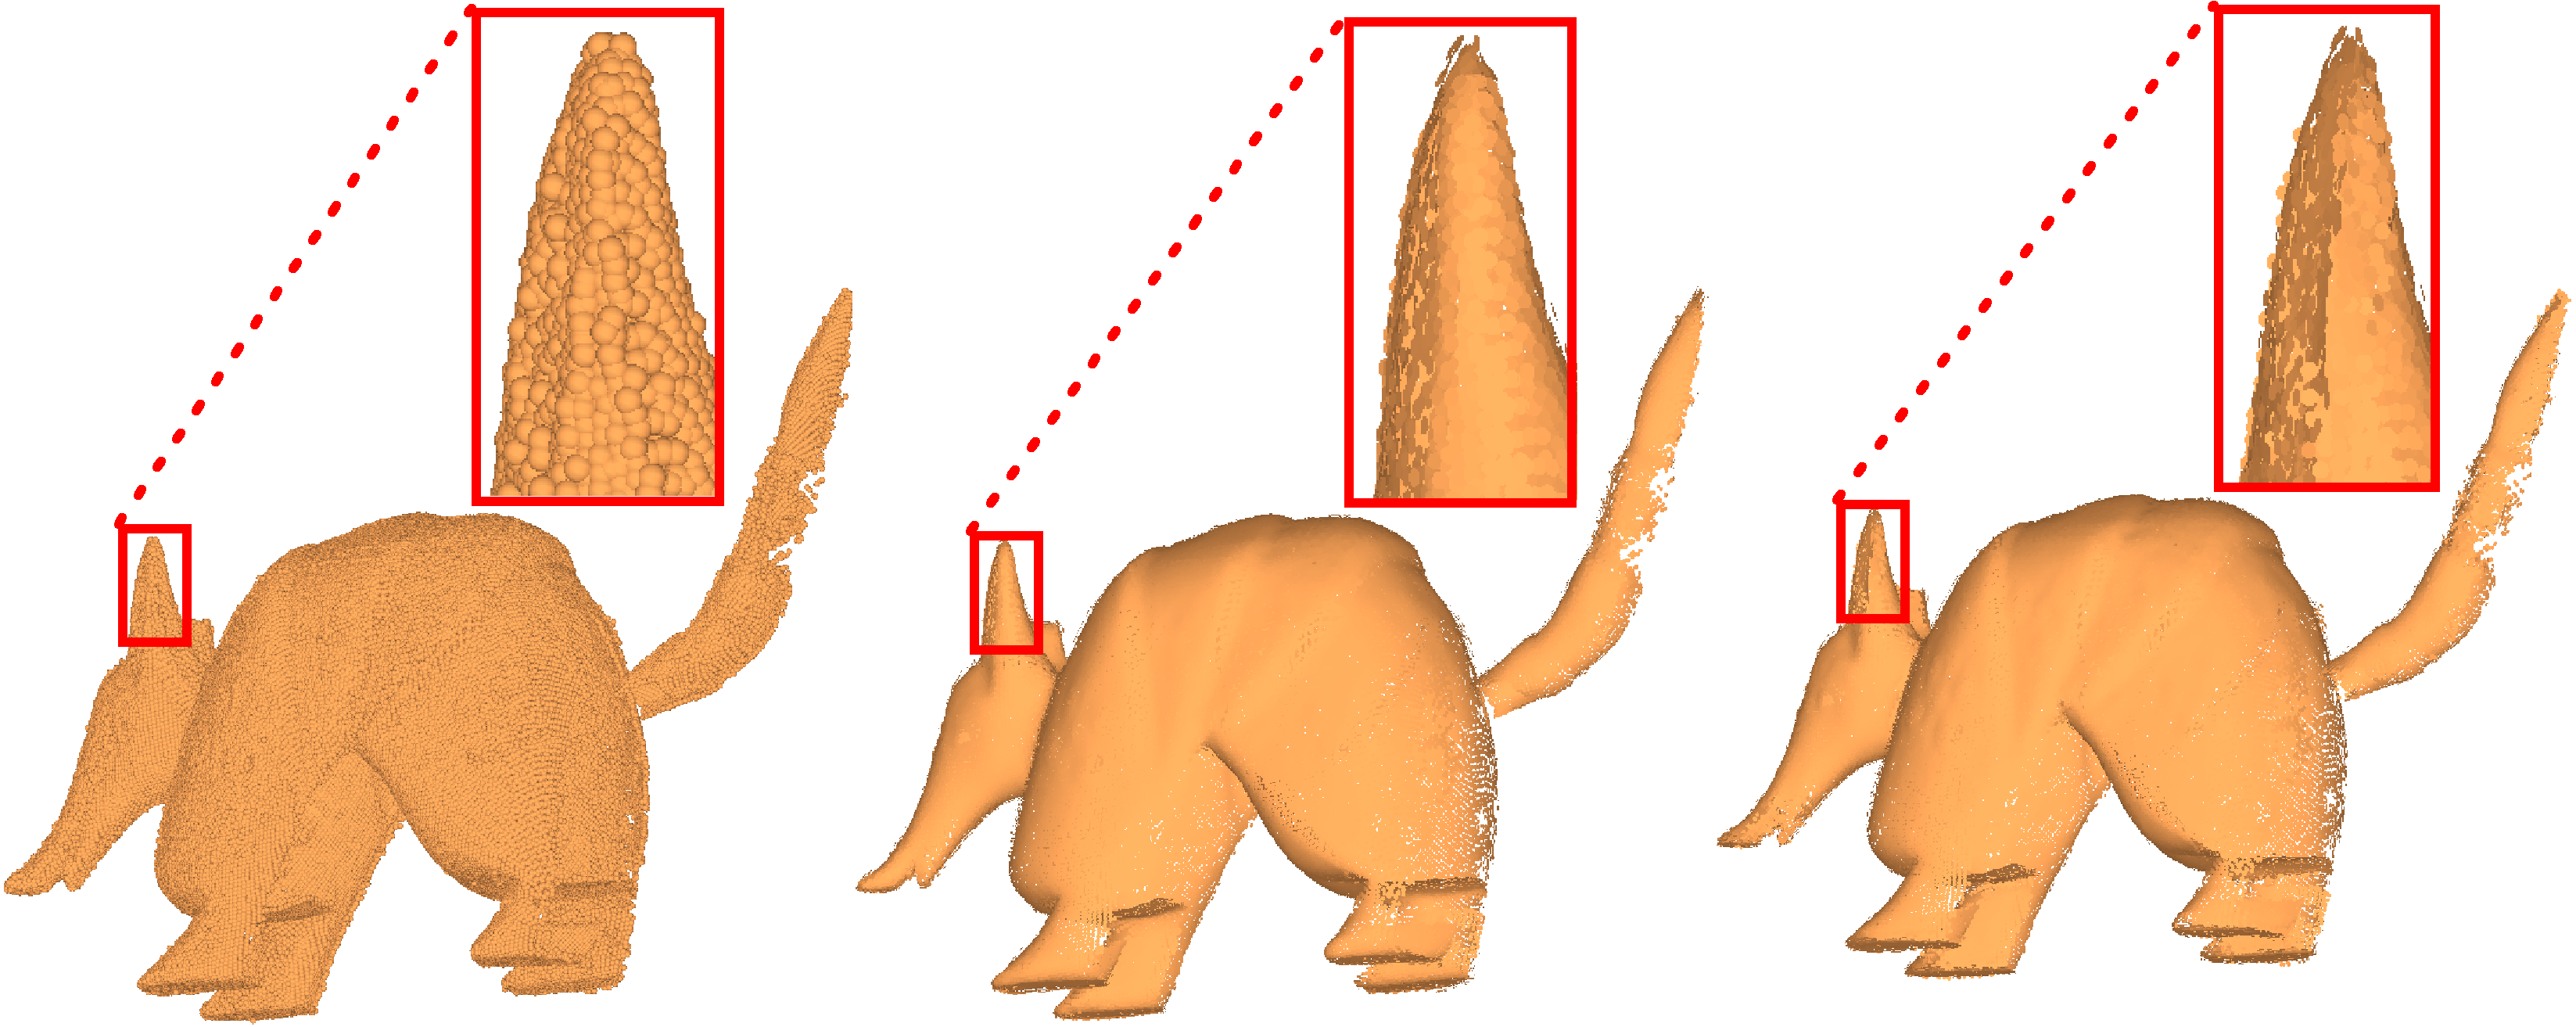
\includegraphics[width=1.0\linewidth]{armadillon}
%    \end{tabular}
%    \caption{{\color{red}Normal estimation results for Armadillon by using PCA and our algorithm. Left to
%     right are the raw scan, the results of PCA and our algorithm, respectively.}\label{fig:armadillo}}
%\end{center}
%\end{figure*}
%\begin{figure*}
%\begin{center}
%    \begin{tabular}{c c }
%        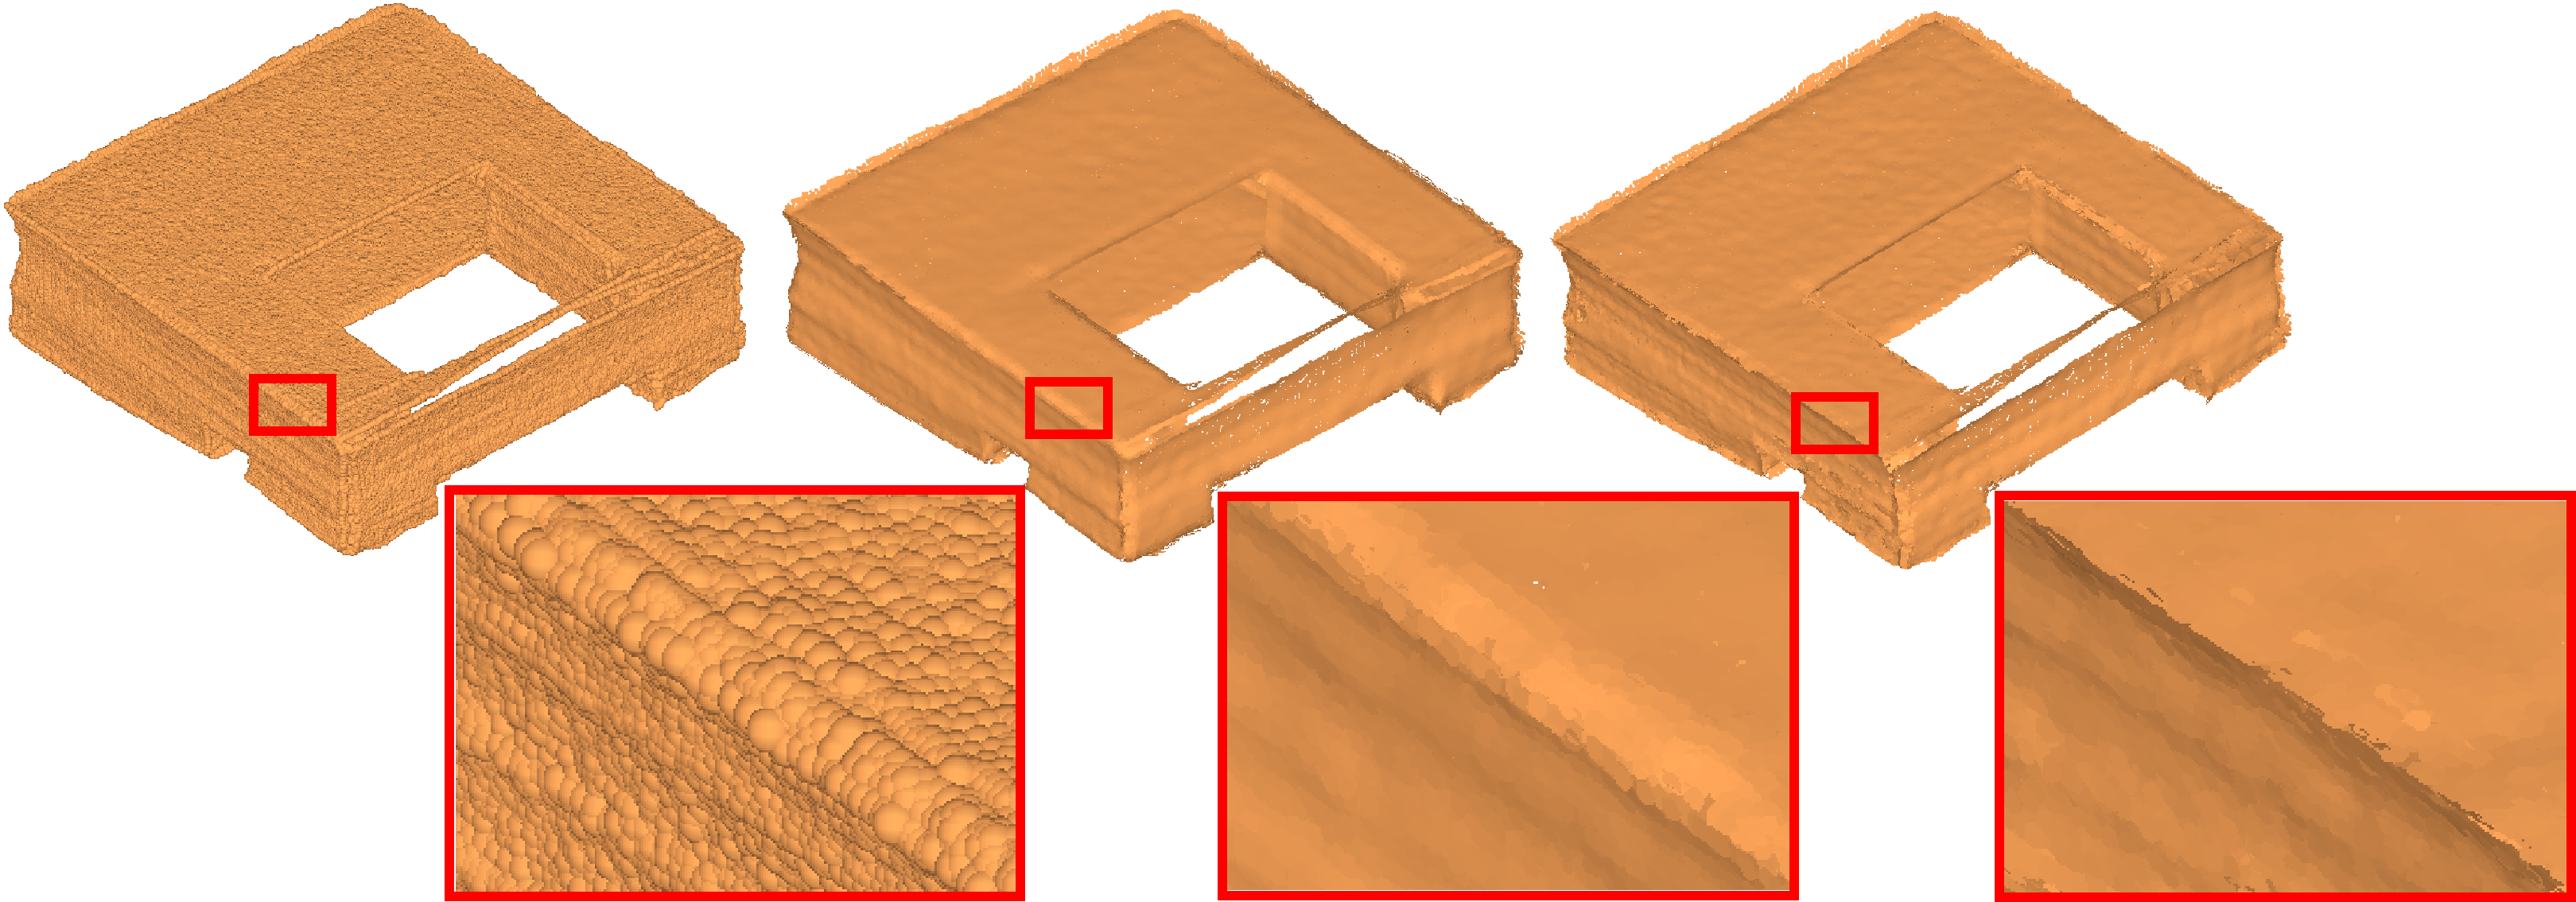
\includegraphics[width=1\linewidth]{box}
%    \end{tabular}
%    \caption{{\color{red}Normal estimation results for Box by using PCA and our algorithm. Left to
%     right are the raw scan, the results of PCA and our algorithm, respectively.}\label{fig:box}}
%\end{center}
\subsection{Implementation details}
\label{sec:implement}
%\textbf{Implementation details.}
The proposed approach has been implemented in Matlab and is not optimized for efficiency. All experiments have been performed with 1 CPU Intel(R) Xeon(R) 2.53GHz.
%
A typical example such as the Armadillon model with 99.4k points and 8.4k candidate feature points in~\fig~\ref{fig:realObjects}, takes a total of 4618 seconds. Of that time, candidate feature points selection, subneighborhood segmentation and normal estimation take 21, 4595 and 2 seconds respectively.
%-
As stated in section~\ref{sec:timing}, the most time-consuming operation is to solve~\eq~(\ref{eq:RSSLRR}) when segmenting subneighborhood of size $S^{*}$ for each candidate feature point.
A parallel C++ implementation with the linearized alternating direction approach \cite{LinLS11} could increase the performance remarkably.

\subsection{Sharp feature detection}

We further demonstrate the effectiveness of our neighborhood segmentation algorithm on sharp feature detection, which is a fundamental problem in geometry analysis.
%
The sharp features are usually detected as the intersection of multiple piecewise smooth surfaces.
%%
%Therefor the intersection of smooth patches produced by can be used to sharp feature detection.
%
Rejecting the pseudo features from real features challenges existing feature extraction methods, since they both are close to the intersection with similar local information, and the difference between the closeness is hard to distinguish.
%
Previous algorithms usually use multi-scale scheme or anisotropic neighborhood selection to extract feature points \cite{PaulyKG03, DanielsHOS07, WeberHH10, ParkLL12}.
%
However, these methods still could not effectively distinguish them by only using distance information.
%
Taking use of the neighborhood segmentation based on subspace structure, we design the following feature extraction method.

%%%%%%%%%%%%%%%%%%%%%%%%%%%%%%%%%%%%%%%%%%%%%%%%%%%%%%
%%%%%%%%%%%%%%%%%%%%%%%%%%%%%%%%%%%%%%%%%%%%%%%%%%%%%%%
%We believe that the true feature points are among the candidate feature points.
%
For each candidate feature point $p_{i}$, we  segment its neighborhood into some subneighborhoods and fit a plane for each.
%
Then we compute the residuals between these fitting planes and $p_{i}$.
%
If there is more than one residual which is less than the threshold $\tau_{feature}$, we consider $p_{i}$ as a feature point.
%
It is worth noting that because we use average residual to define the $\tau_{f}$, we set $\tau_{feature} = 2 \times \tau_{f}$.


%%%%%%%%%%%%%%%%%%%%%%%%%%%%%%%%%%%%%%%%%%%%%%%%%%%%%%
%%%%%%%%%%%%%%%%%%%%%%%%%%%%%%%%%%%%%%%%%%%%%%%%%%%%%%%
To assess the quality of sharp features detected by the method, we test it on synthetic models with random noise and compare it with the recent work~\cite{ParkLL12} (MSTV).
%
%Since the noise of feature detection is usually smaller than normal estimation,
The parameters $S$, $S^{*}$, $K$ and $r$ of our algorithm are choose as $S=20$, $S^{*}=60$, $K=10$ and $r=4$ for all tests in this section.

%\begin{figure}[htbp]
%\begin{center}
%    \begin{tabular}{c c c}
%        \includegraphics[width=0.3\linewidth]{fandisk_00} &
%        \includegraphics[width=0.3\linewidth]{ploy_original_343_409} &
%        \includegraphics[width=0.33\linewidth]{flower_original_343_409}\\
%        \includegraphics[width=0.3\linewidth]{fandisk_00_f} &
%        \includegraphics[width=0.3\linewidth]{ploy_feature_343_409} &
%        \includegraphics[width=0.33\linewidth]{flower_feature_343_409}
%    \end{tabular}
%    \caption{Sharp feature detection results.\label{fig:noise_free_feature}}
%\end{center}
%\end{figure}
\begin{figure}[htbp]
\begin{center}
    \begin{tabular}{c c c}
        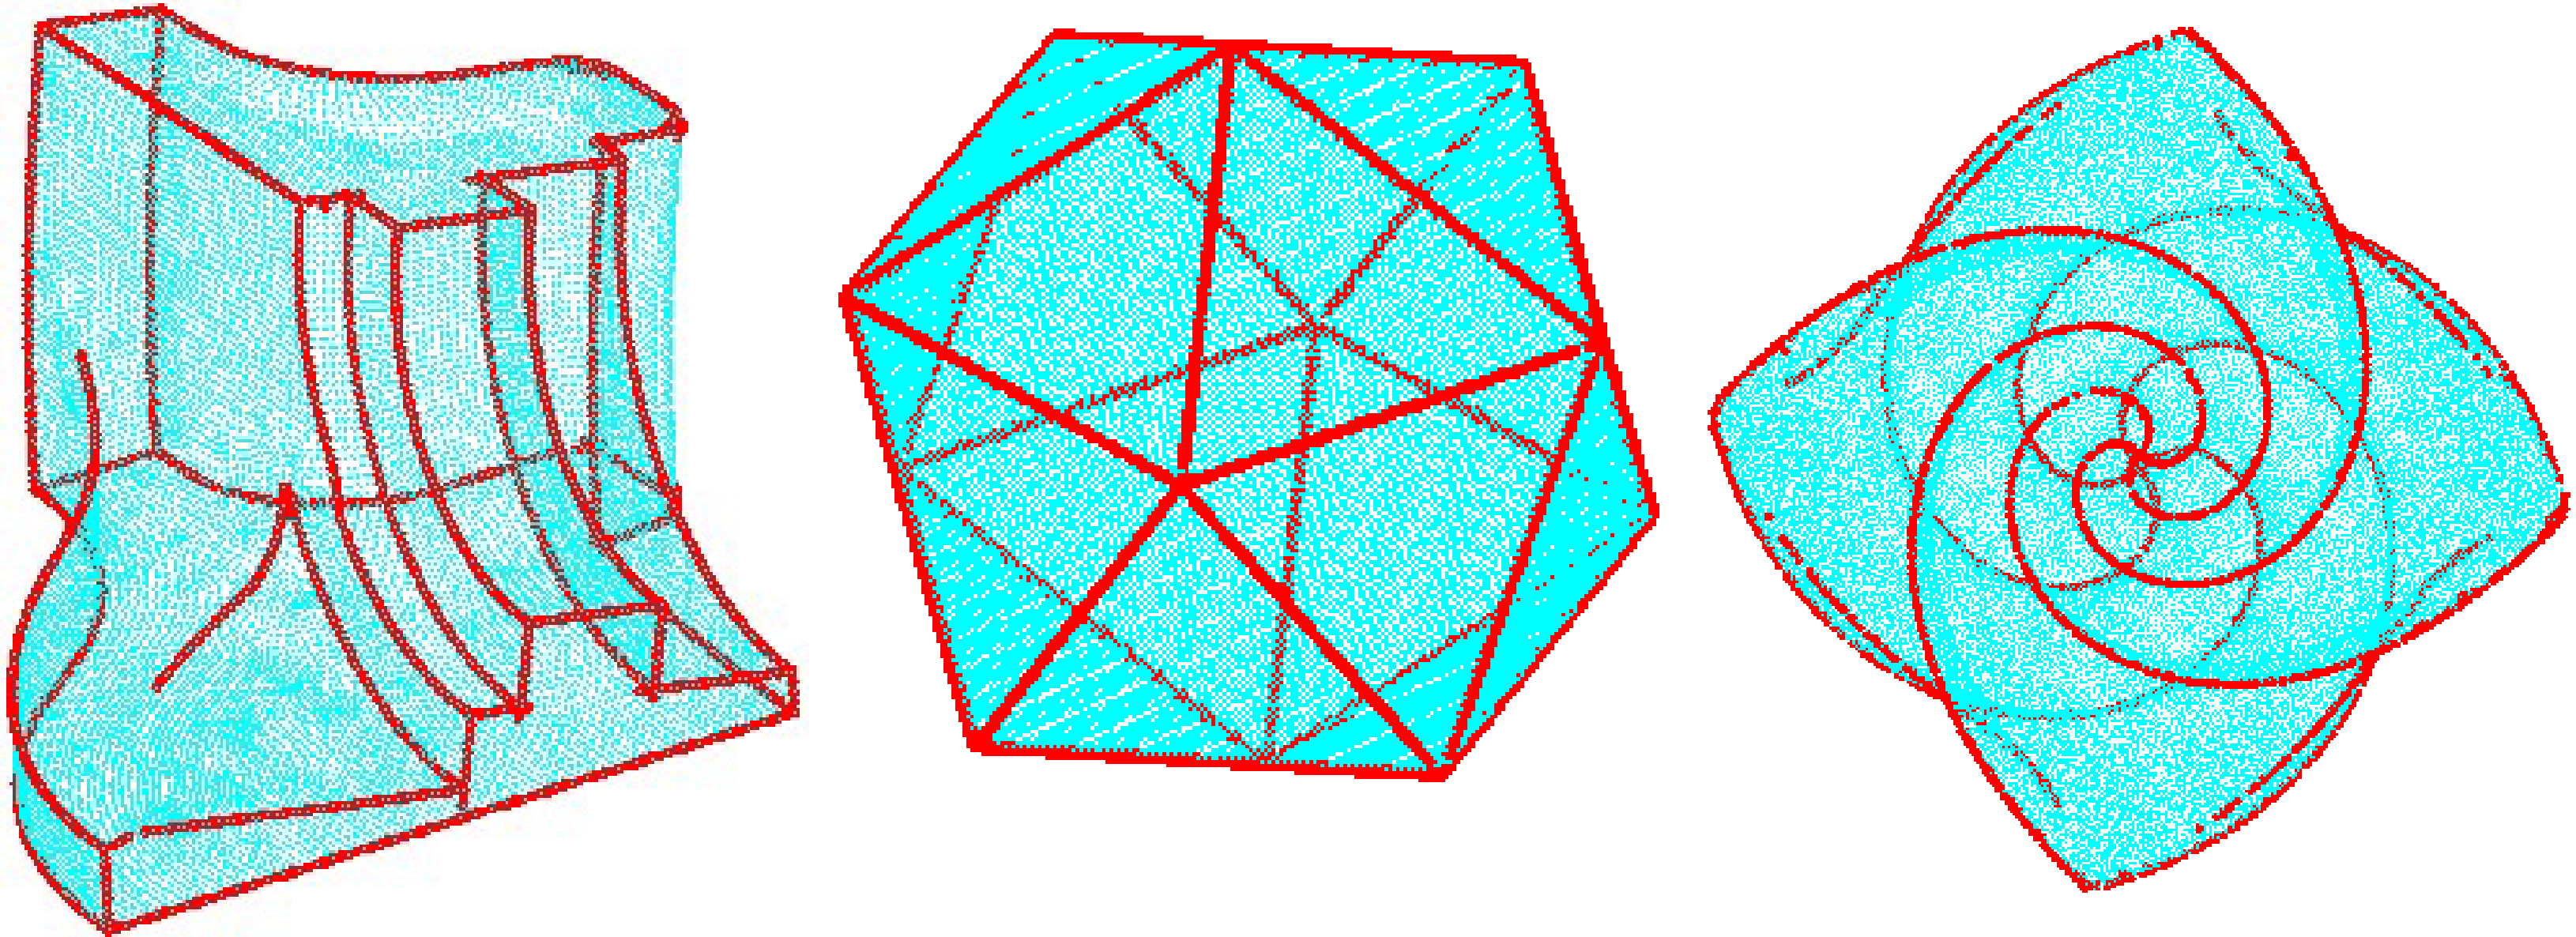
\includegraphics[width=1\linewidth]{noise_clear_feature}
    \end{tabular}
    \caption{Sharp feature detection results.\label{fig:noise_free_feature}}
\end{center}
\end{figure}
Detection results of three different models are show in Fig. \ref{fig:noise_free_feature}.
%
For these noise-free models, our method achieves almost perfect detection results, although the shapes are complex. There are Fandisk model, Icosahedron model which has corners with five adjoining planes, and Flower model where sharp features are jaggy.
%although the shapes in Fig. \ref{fig:noise_free_feature} are complex. There are \jj{...}. \jj{remove figure for weak feature}
%
We can see that our method can detect the weak features well, especially in the Flower model.


%%%%%%%%%%%%%%%%%%%%%%%%%%%%%%%%%%%%%%%%%%%%%%%%%%%%%%
%%%%%%%%%%%%%%%%%%%%%%%%%%%%%%%%%%%%%%%%%%%%%%%%%%%%%%%
In order to demonstrate the robustness of our method to noise, the results of Fandisk and Smooth-feature models are shown in \fig \ref{fig:noise} and \fig \ref{fig:compare_feature}, which are perturbed by centered Gaussian noise with the standard deviation of $10\%$ and $20\%$ average distance between points, respectively.
%Our method is robust against noise, as shown in \fig \jj{? and ?}.
%Two scales of centered Gaussian noise with the standard deviation of $10\%$ and $20\%$ average distance between points are added to the Fandisk and ? models.
%
As illustrated in \fig \ref{fig:noise}, our method is able to detect the sharp features in different noise scale for the Fandisk model.
%
Moreover, the weak features are recovered perfectly.
%
The visual comparison between the recent method MSTV and our method is given in
\fig \ref{fig:compare_feature}.
%
MSTV can not restore weak features perfectly and some weak feature points at the top of the model are missing, as shown on the top of  \fig \ref{fig:compare_feature}.
%
%The results provided by Park et al. \jj {per} are shown in Fig. \jj {fig} and \jj {fig}.
%
%The method of \jj {fig} could not restore weak features perfectly and some weak feature vertices at the top of the model are missing.
%
While evidence from the bottom of~\fig~\ref{fig:compare_feature} demonstrates that our method is capable of recovering more weak feature points to a large extent.

\begin{figure}[htcb]
  \centering
  \begin{tabular}{c c c c}
        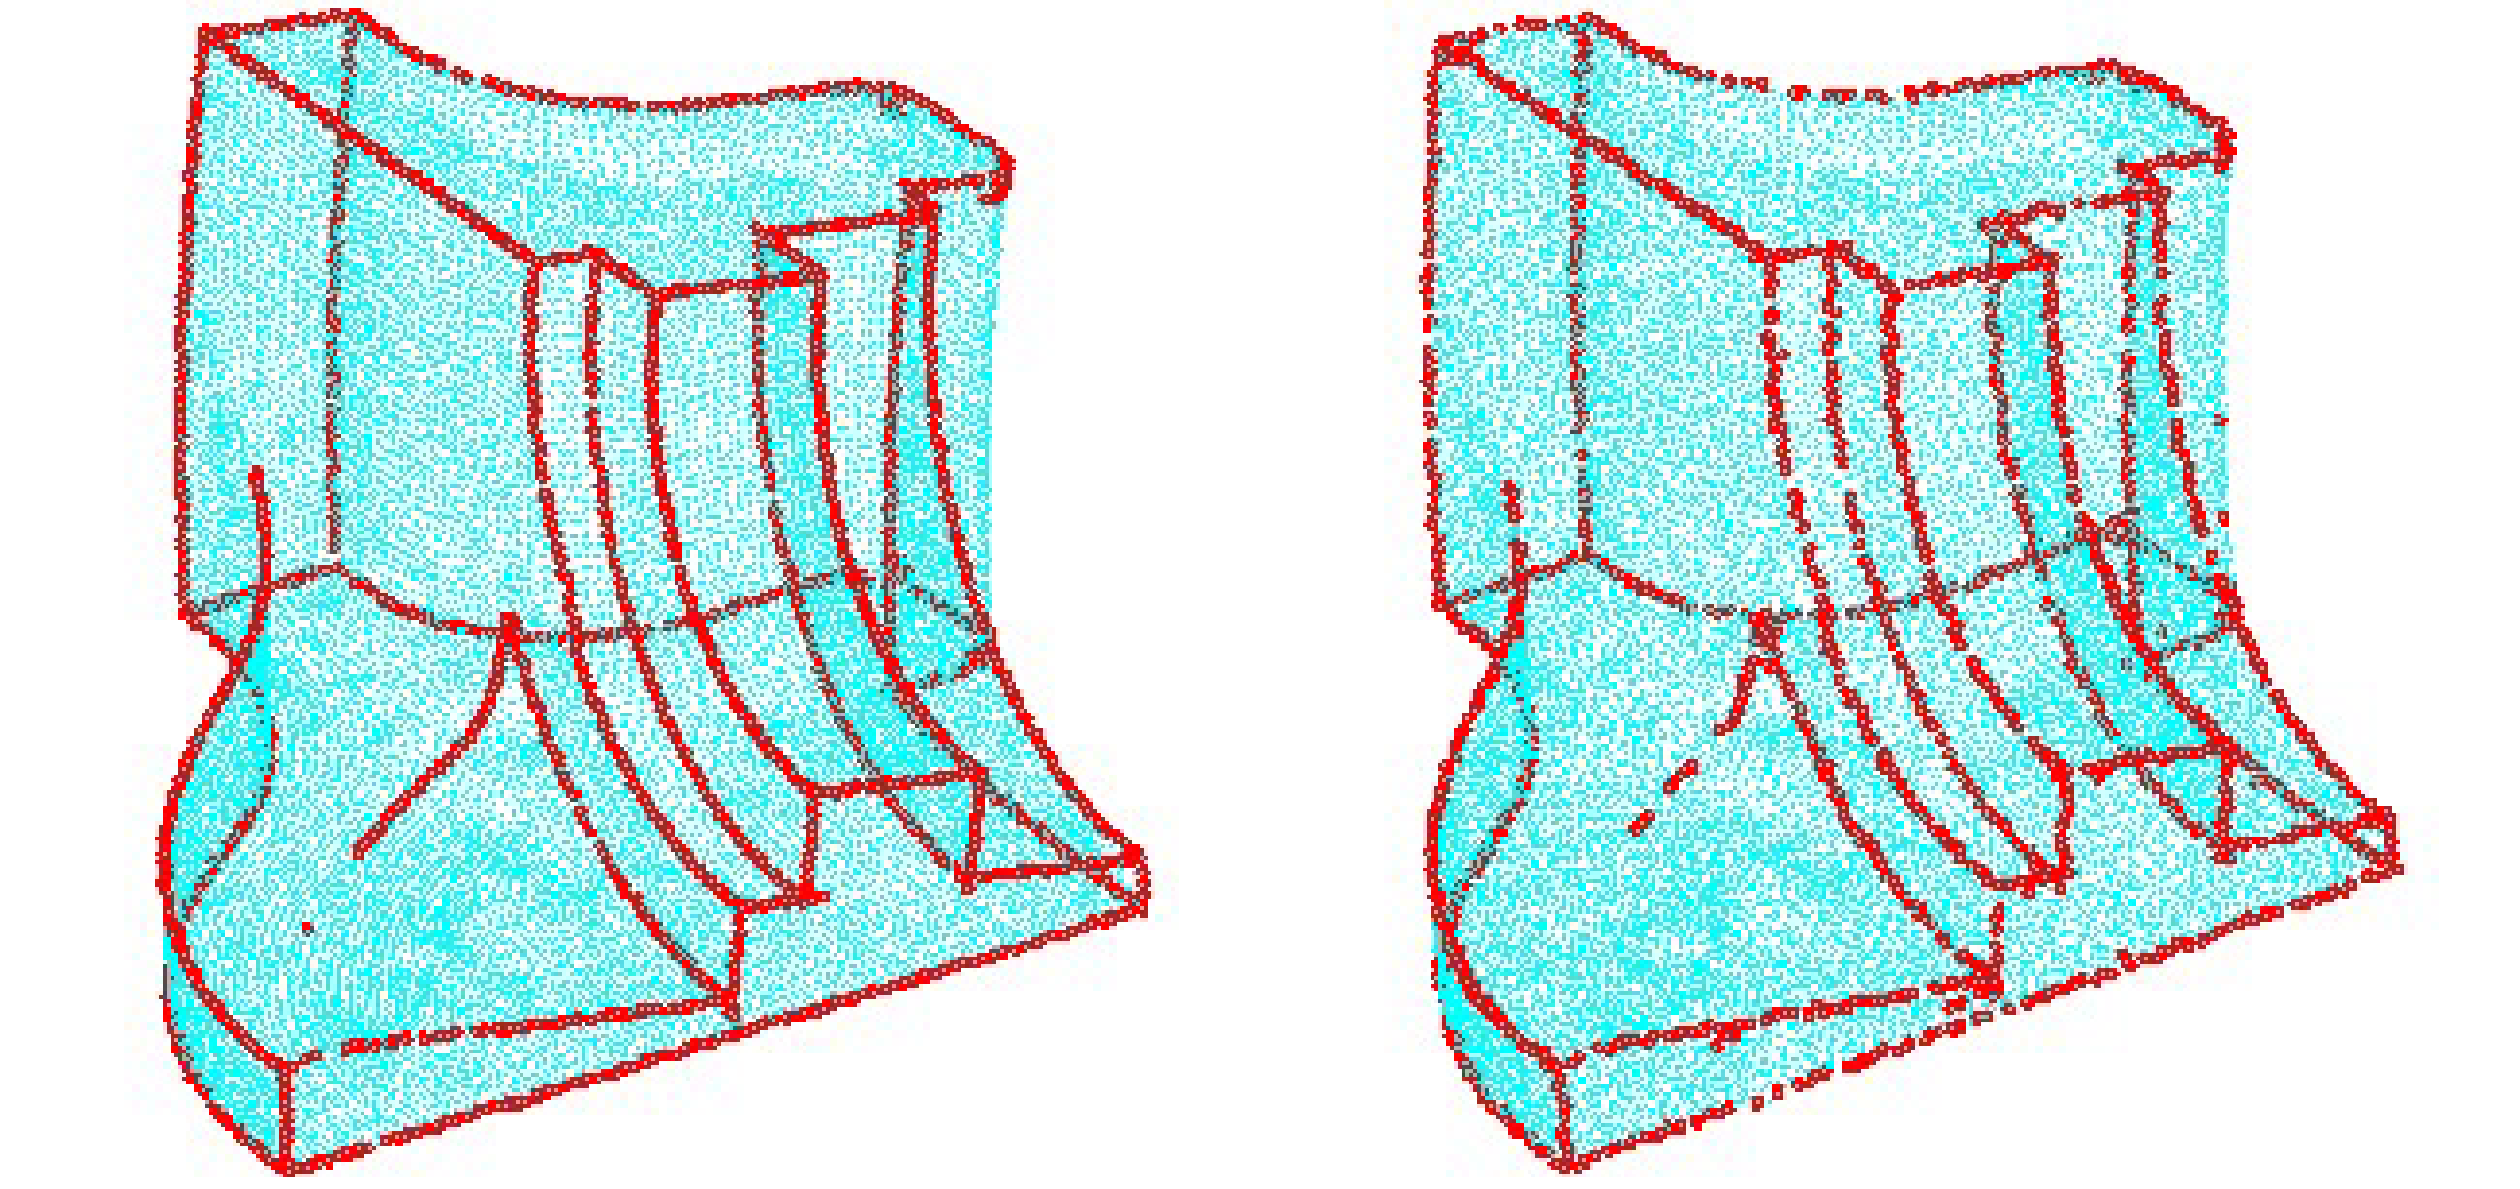
\includegraphics[width=1\linewidth]{fandisk_noise}
    \end{tabular}
  \caption{\label{fig:noise}
   Sharp feature detection results for the Fandisk model with $10\%$ (left) and $20\%$ (right) Gaussian noise.
   }
\end{figure}
\begin{figure}[htbp]
\begin{center}
    \begin{tabular}{c c }
        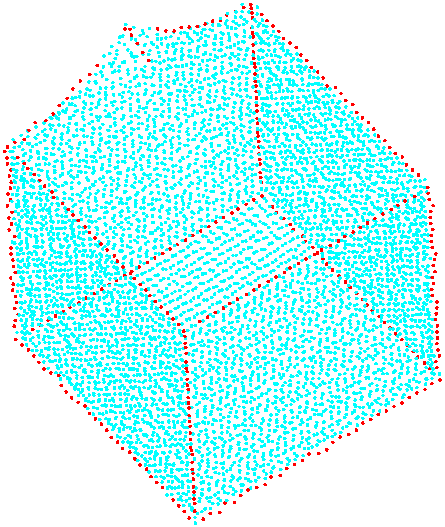
\includegraphics[width=0.4\linewidth]{smooth_10_mv} &
        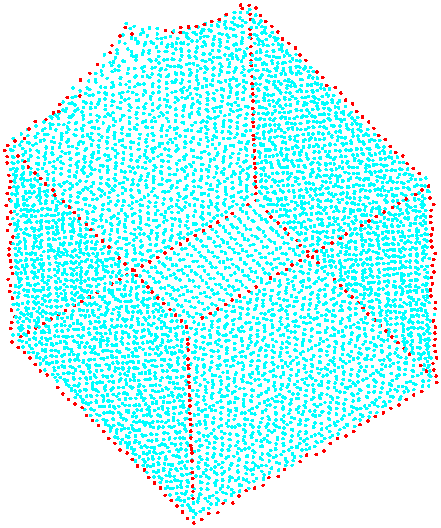
\includegraphics[width=0.4\linewidth]{smooth_20_mv} \\
        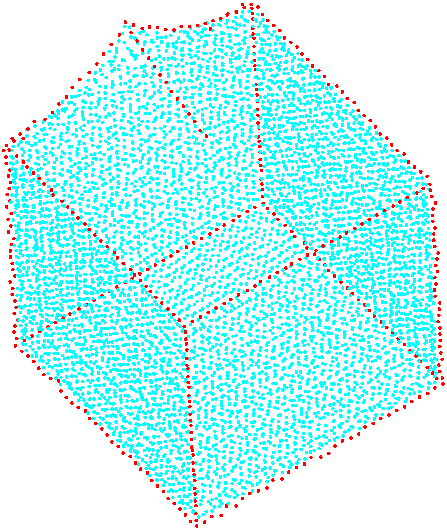
\includegraphics[width=0.4\linewidth]{smooth_10_our} &
        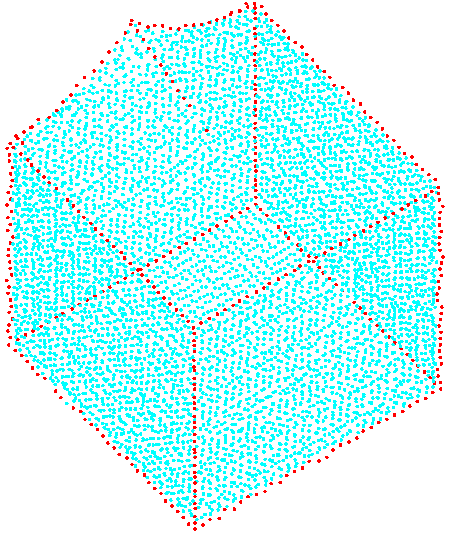
\includegraphics[width=0.4\linewidth]{smooth_20_our}
    \end{tabular}
    \caption{The sharp feature detect results by MSTV (top) and our method (bottom). Left: Smooth-feature model with $10\%$ Gaussian noise. Right: Smooth-feature model with $20\%$ Gaussian noise. \label{fig:compare_feature}}
\end{center}
\end{figure}

%-------------------------------------------------------------------------
\section{Conclusion}
Motivated by the observation that the segmentation of the neighborhood of the point near sharp features can be treated as subspace clustering, we propose a novel normal estimation method for point clouds, which is able to preserve sharp features even in the presence of heavy noise.
%We have proposed a novel method for estimating normals for point clouds that preserves sharp features and that is robust to noise and outliers.
%
In order to obtain more stable segmentation, a more general LRR framework for subspace clustering with guidance from prior knowledge is presented. We also design an unsupervised learning process to estimate the guidance from reliable regions for the purpose of normal estimation.
%
The experiments exhibit that our method is more resilient to noise than state-of-the-art methods.
%We have shown that our method is at least as precise and noise-resistant as state-of-the-art methods that preserve sharp features,
%
Moreover, it is robust to non-uniform sampling that is a more challenging issue in normal estimation.
%
\re{It would also be interesting to apply our guided low-rank subspace clustering framework to more computer vision and computer graphics applications.}


\re{As described in Section \ref{sec:algorithm}, our method requires a substantial amount of computation time to solve ~\eq~(\ref{eq:RSSLRR}) at each candidate feature point. In the future, we try to find a more efficient algorithm to solve~\eq~(\ref{eq:RSSLRR}) and design a parallel implementation for our normal estimation method.
%
Another future work is to choose the four parameters $S$, $S^{*}$, $K$ and $r$ adaptively according to noise level and sampling density.
}
%
%(the previous version) As future work, it would be interesting to choose the four parameters $S$, $S^{*}$, $K$ and $r$ adaptively according to noise level and sampling density. Another future work may be apply our method to more feature-preserving applications.

%One limitation of our method may be the computational time. It usually takes hours for models with tens of thousands of points in our current Matlab implementation. We plan to accelerate our algorithm from two aspects: strategy of avoiding to segment neighborhood of each candidate feature points and rapid computation method for reducing the computation time.

\section*{Acknowledgement}
The authors would like to thank all the reviewers for their valuable comments.
%
This work is partially supported by the National Natural Science Foundation of China (No. 61173102, U0935004, 61173103, 91230103) and the Research Funds for the Central Universities (No. DUT13RC206, DUT13JS04).
%
Thanks to Bao Li and Alexandre Boulch for providing the code used for comparison.
%
The Armadillon model is courtesy of Andrei Sharf. The models of Box and Shutter are provided by Hui Huang.
%-------------------------------------------------------------------------
%\section{References}

\bibliographystyle{elsarticle-num}
\bibliography{smi_template}
\appendix
\section{Solving of LRSCPK}


Alternating Direction Method (ADM) \cite{convergence} is used to solve ~\eq~(\ref{eq:RSSLRR}). First, by introducing two auxiliary variables,~\eq~(\ref{eq:RSSLRR}) can be written as
\begin{equation}
\begin{array}{l}
\label{eq:defineS1}
min_{Z,E}\|J\|_{*}+\beta\|\mathcal{P}_{\Omega}(L)\|_{1}+\gamma\|E\|_{2,1},\\
s.t. X=XZ+E, Z=J, Z=L.
\end{array}
\end{equation}
Then the problem can be solved by minimizing the following augmented lagrange function
\begin{equation}
\begin{array}{l}
\label{eq:defineSau}
\|J\|_{*}+\beta\|\mathcal{P}_{\Omega}(L)\|_{1}+\gamma\|E\|_{2,1}+\langle Y^{B},Z-L\rangle\\
+\langle Y^{A},X-XZ-E\rangle + \langle Y^{C},Z-J\rangle + \frac{\mu}{2}(\\
\|Z-J\|_{F}^{2}+\|X-XZ-E\|_{F}^{2}+\|Z-L\|_{F}^{2}),
\end{array}
\end{equation}
where $Y^{A}$, $Y^{B}$ and $Y^{C}$ are lagrange multipliers. We outline the procedure of the algorithm in Algorithm \ref{alg:Framwork1}. The closed-form solutions of step 1 and step 4 can be solved via Soft Value Thresholding (SVT) operator \cite{CaiCS10} and the Lemma 3.2 in \cite{LiuLY10}, respectively.

\begin{algorithm}[htb] %�㷨�Ŀ�ʼ
\renewcommand{\algorithmicrequire}{\textbf{Input:}}
\renewcommand\algorithmicensure {\textbf{Initialize:} }
\caption{Solving ~\eq~(\ref{eq:RSSLRR}) by ADM}
\label{alg:Framwork1} %���㷨һ����ǩ���������������ж��㷨������
\begin{algorithmic} %���1 ��ʾÿһ�ж���ʾ����
\REQUIRE matrix $\mathbf{X,\Omega}$, parameter $\beta$ and $\gamma$
\ENSURE $\mathbf{Z=J=L=0}$, $\mathbf{E=0}$,
$\mathbf{Y}^{A}=\mathbf{Y}^{B}=\mathbf{Y}^{C}=0$, $\mu=10^{-6}$,
$max_{\mu}=10^{6}$, $\rho=1.1$, $\varepsilon=10^{-8}$. \WHILE{not
converged}
\STATE 1. Fix the others and update $\mathbf{J}$\\
$\mathbf{J}=argmin\frac{1}{\mu}\|\mathbf{J}\|_{*}+\frac{1}{2}\|\mathbf{J}-(\mathbf{Z}+\frac{\mathbf{Y}^{C}}{\mu})\|_{F}^{2}.$
\STATE 2. Fix the others and update $\mathbf{L}$\\
$\mathbf{L}=argmin\frac{\beta}{\mu}\|\mathcal{P}_{\Omega}(\mathbf{L})\|_{1}+\frac{1}{2}\|\mathbf{L}-(\mathbf{Z}+\frac{\mathbf{Y}^{B}}{\mu})\|_{F}^{2}.$
\STATE 3. Fix the others and update $\mathbf{Z}$\\
$\mathbf{Z}=(2\mathbf{I}+\mathbf{X}^{T}\mathbf{X})^{-1}(\mathbf{X}^{T}(\mathbf{X}-\mathbf{E}+\frac{\mathbf{Y}^{A}}{\mu})+\mathbf{J}+\mathbf{L}-\frac{\mathbf{Y}^{C}}{\mu}-\frac{\mathbf{Y}^{B}}{\mu}).$
\STATE 4. Fix the others and update $\mathbf{E}$\\
$\mathbf{E}=argmin\frac{\gamma}{\mu}\|\mathbf{E}\|_{2,1}+\frac{1}{2}\|\mathbf{E}-(\mathbf{X}-\mathbf{XZ}+\frac{\mathbf{Y}^{A}}{\mu})\|_{F}^{2}.$
\STATE 5. Update the multipliers\\
$\mathbf{Y}^{A}=\mathbf{Y}^{A}+\mu(\mathbf{X}-\mathbf{XZ}-\mathbf{E})$, $\mathbf{Y}^{B}=\mathbf{Y}^{B}+\mu(\mathbf{Z}-\mathbf{L})$, $\mathbf{Y}^{C}=\mathbf{Y}^{C}+\mu(\mathbf{Z}-\mathbf{J})$.  \STATE 6. Update the parameter $\mu$\\
 $\mu=min(\rho\mu,max_{\mu})$. \STATE 7. Check the convergence conditions \\
$\|\mathbf{X}-\mathbf{XZ}-\mathbf{E}\|_{\infty}<\varepsilon$,
$\|\mathbf{Z}-\mathbf{J}\|_{\infty}<\varepsilon$,
$\|\mathbf{Z}-\mathbf{L}\|_{\infty}<\varepsilon$.\ENDWHILE
\end{algorithmic}
\end{algorithm}




%-------------------------------------------------------------------------
%\newpage
%
%\mbox{}
%\newpage
%
%\mbox{}
%\newpage
%
%\begin{center}
%       \LARGE{Rebuttal}
%\end{center}
%\bl{We would like to thank all the reviewers for their thoughtful comments. We shall first make a few points intended for all the reviewers. Responses (colored blue) to individual reviewer comments will follow. In the current revision, included changes are colored red.

One main issue raised by the reviewers is that our work is mostly based on existing work.
%-
As stated in Section 1 and 3, the existing Low-Rank Subspace Clustering methods tend to fail when segmenting two or more intersection planes, i.e. when the subspaces are dependent. In this paper, we present a low-rank based framework with prior knowledge for more general subspace clustering. The framework has the potential to be employed in many other computer vision and graphics applications when the subspaces are not independent.

The second common issue is about timing.
%-
The time complexity of our algorithm is $O(N\mathrm{log}N + N_{f}\times (S^{*})^{3})$, where $N$ is the number of points and $N_{f}$ is the number of the candidate feature points.
Solving ~\eq~(\ref{eq:RSSLRR}) is the most time-consuming (the $(S^{*})^{3}$ factor), which can be reduced to $O((S^{*})^{2})$ using the linearized alternating direction approach \cite{LinLS11}.
We have added Section~\ref{sec:timing} for time complexity analysis and offered a typical timing for
the Armadillon model with 99.4k points and 8.4k candidate feature points in~\fig~\ref{fig:realObjects}. It takes a total of 4618 seconds using our current Matlab implementation. A parallel C++ implementation with the linearized alternating direction approach could increase the performance remarkably.

The third issue is about more "real-life" examples.
%-
We have added a few more real-scan data in~\fig~\ref{fig:realObjects} and~\fig~\ref{fig:shutter}, in which the typical imperfections, such as noise, outliers and non-uniform distribution are ubiquitous.
Necessary comments are added in Section~\ref{sec:moreResults}.
%-
The facade model in Fig. 2 of original manuscript is removed since it takes too much of space.

The last issue is about display.
%-
The surfels for sharp features (clipped two disks) [21] may not be a proper approach for display normals before feature edges are extracted. One of the author of [21] refers us to Pointshop3D which is not supported after December 2006. We are studying the code still. In the current revision, we have tried hard to improve the display by adjusting the size of the surfels.
}

%-------------------------------------------------------------------------
\vspace{10pt}

\noindent
{\bf Reviewer \#1}

\vspace{10pt}

\noindent
Comment 1:
Since computer graphics people seems not to be so familiar with computer vision techniques, thus the numerical method solving the optimization in Equation (6) needs to be briefly explained (if the extra space exists).

\noindent
\bl{Response: We adapt Alternating Direction Method (ADM) to solve Equation (6) which is detailed in Appendix 1.
}

%-------------------------------------------------------------------------
\vspace{10pt}

\noindent
Comment 2: It is better to mention what is the meaning "RNE" and "HF".

\noindent
\bl{Response: "RNE" means robust normal estimation, and "HF" means hough transform. We have rewrote the first paragraph of Section~\ref{sec:results}.
}

%-------------------------------------------------------------------------
\vspace{10pt}

\noindent
Comment 3: "Alexandre" is the first name. The method proposed in [7] is explained two times.

\noindent
\bl{Response: Corrected. Thank you.
}

%-------------------------------------------------------------------------
\vspace{10pt}

\noindent
Comment 4: The same procedure for computing $w_i$ is introduced in Mark Pauly, Markus Gross, Leif Kobbelt, "Efficient Simplification of Point-Sampled Surfaces",IEEE Visualization 2002. In Equation (7), $T->T_i$, and $s->S$.

\noindent
\bl{Response: We have simplified the introduction of $w_i$ by citing \cite{PaulyKKG03}, and Equation (7) is also removed, see the first paragraph of Section \ref{subsec:candidateFeature}.
}

%-------------------------------------------------------------------------
\vspace{10pt}

\noindent
Comment 5: Please provide the reference for "$l_1$-smoothed distribution".

\noindent
\bl{Response: We have detailed the process in the last paragraph of Section \ref{subsec:candidateFeature}.
}

%-------------------------------------------------------------------------
\vspace{10pt}

\noindent
Comment 6: In Section 4.3.2, what is the meaning "edge" ? Is it same as "sharp feature" ?

\noindent
\bl{Response: They are the same meaning. To avoid unnecessary misleading, we have replaced edge with sharp feature.
}

%-------------------------------------------------------------------------
\vspace{10pt}

\noindent
Comment 7: In Equation (8), root mean square is represented as "RMS", but in the other "RSM" is used.

\noindent
\bl{Response: Corrected.
}

%-------------------------------------------------------------------------
\vspace{10pt}

\noindent
Comment 8: Could you explain the reason why the parameters S, S*, K, and r are different in normal estimation and feature extraction ?

\noindent
\bl{Response: We chose smaller neighborhood just for speeding up the algorithm.
}


%-------------------------------------------------------------------------
\vspace{10pt}

\noindent
Comment 9: References [6] and [17] are same. The authors and title are missing for [26].

\noindent
\bl{Response: Corrected.
}

%-------------------------------------------------------------------------
\vspace{10pt}

\noindent
{\bf Reviewer \#3}

\vspace{10pt}

\noindent
Comment 1:
It is mandatory that all these info are added to the paper.
For example in the following paper (that probably should be cited) the authors take into account performance in the evaluation of various surface normal estimation methods.
Klasing, K.; Althoff, D.; Wollherr, D.; Buss, M., "Comparison of surface normal estimation methods for range sensing applications," Robotics and Automation, 2009. ICRA '09. IEEE International Conference on , vol., no., pp.3206,3211, 12-17 May 2009

\noindent
\bl{Response: These info are provided, as shown in the common concern section above. We also cited the paper because it adds to our related work description by evaluating the performance of various normal estimation methods.
}

%-------------------------------------------------------------------------
\vspace{10pt}

\noindent
{\bf Reviewer \#4}

\vspace{10pt}

\noindent
Comment 1: I didn't have time to completely check all the mathematical details but it seems to be correct. However, a self contained explanation is desirable.

\noindent
\bl{Response: Many detailed descriptions have been added accordingly. We introduced Sparse subspace clustering and Low-rank subspace clustering in Section \ref{sec:lowrank} before introducing our LRSCPK. The most important merit of LRSCPK is that it handles the subspace clustering problem when the subspaces are dependent which challenges the classical low rank subspace clustering approaches. The guiding matrix provides a constraint such that the representation with the same class is dense and that of different classes is sparse as explained in Section \ref{sec:LRSCPK}. The toy example in Section \ref{sec:toy} also provides an intuitive illustration.
}

%-------------------------------------------------------------------------
\vspace{10pt}
\noindent
Comment 2: Since the theory of low-rank subspace clustering is quite new, I recommend a presentation with more details.

\noindent
\bl{Response: It is really a challenge to add more about low-rank subspace clustering since 14 pages is the upper limit of SMI paper. Section \ref{sec:subspacesegmentation} and \ref{sec:LRSC} provide necessary introduction about the motivation, model and defect of low-rank subspace clustering. More info can be found in~\cite{DBLP:journals/corr/abs-1010-2955} and ~\cite{DBLP:conf/cvpr/ElhamifarV09}.
}

%-------------------------------------------------------------------------
\vspace{10pt}
\noindent
Comment 3: I recommend  figure 4 to be placed in the introduction. I think that presenting an overview in the beginning of the paper is more attractive. Again, as in the figure 2, figure 4(d) does not give any information.

\noindent
\bl{Response: We have move it in the introduction. In the figure, (a) is the input model with normal estimated by PCA and (d) is our result which preserving the sharp features better as highlighted by the two green boxes. We also showed the $RMS\_\tau $ of them.
}

%-------------------------------------------------------------------------
\vspace{10pt}
\noindent
Comment 4: The comparison with other methods must be done carefully. Since there are many parameters to be controlled, the authors should be sure that they are set in the best performance.

\noindent
\bl{Response: The parameters are carefully tuned according to the descriptions of authors of HF and RNE. We have tried our best to choose them after many times of experiments. The authors of RNE have confirmed the results we computed.
}

% \newpage


\end{document}
